%%% Kapitoly
\chapter{Experimenty}
Všechny práce zmíněné v úvodní kapitole, sice používají evoluční algoritmy k vytvoření řízení chování homogenního robotického hejna, tzn. s jedním druhem robotů. V následující kapitole podrobně popíši postup hledání optimální chování pro heterogenního hejna. Optimalizaci jsem navrhl a otestoval na třech rozličných scénářích. Hlavní motivací při tvorbě scénářů bylo vytvořit obtížnější úkoly než se obvykle používají jako například: shlukování, vyhýbání překážkám... Navrhnout je natolik komplexně, aby nebylo možné, že část hejna se nebude podílet na jeho plnění. Také jsem volil scénáře, aby se přiblížily situacím z reálného světa. Každému z nich jsem věnoval samostatnou kapitolu, která zahrnuje popis hlavního úkolu scénáře, seznam robotů i s jejich senzory a efektory, způsob hodnocení fitness,rozdělení do podúkolů s průběhem fitness u ES a DE, vizualizaci a rozbor chování nejlepšího jedince.  
\subsubsection{Pracovní názvy scénářů:}
\begin{enumerate}
	\item Wood Scene - zpracování dřeva
	\item Mineral Scene - přetvoření minerálů na palivo 
	\item Competitive Scene - soubojový scénář
\end{enumerate}
\par
Pro řešení problému jsem navrhl řadu postupů, proto v tomto odstavci zmíním ty nejvíce přímočaré a slibné, které se ovšem ukázaly  jako neúspěšné. V kapitolách zabývajícími se konkrétními scénáři už budu pouze popisovat jen konečné, úspěšné postupy.
 \par
 \improvement{Přidat další podrobnosti o fitness}
Nedostatečný se ukázal pokus provádět evoluci pro fitness hlavního úkolu scénáře. Většina hodnocení náhodných chování byl roven nule, proto EA nedostaly dostatek informací k vhodné exploraci a díky malé pravděpodobnosti vygenerování chování alespoň částečně řešící hlavní úkol nedocházelo ani k exploataci. Což mělo za důsledek neefektivní  DE a ES, takže ani jeden z EA nedošel k úspěšnému řešení. 
\par
Posun zaznamenala více obecná fitness i když sama o sobě také nedosáhla do kategorie úspěšných postupů. Do fitness jsem zahrnul i menší pozitivní znaky, které byly součástí hlavnímu úkolu. Například jsem záporně ohodnotil pokusy o pohyb končící kolizí, kladně počet nalezených entit či vhodných objektů v kontejnerech, aktuální stav paliva. Optimalizovaná chování opravdu zaznamenala posun. Ovšem oba EA obtížně hledaly cestu z lokálního optima a ve většině případů optimalizovali pouze jednoduché části úkolu. I přes přidávání složitějších matematických funkcí do fitness nebyly schopny dosáhnout uspokojivého řešení hlavního úkolu scénáře. 
\par 
Pro finální řešení jsem zvolil metodu, kterou nazývám metodou podúkolů. U každého scénáře podrobně popíši její průběh a nastavení, zde pouze nastíním základní  myšlenku. Rozdělil jsem hlavní cíl na několik menších podúkolů (metaúkolů). Každému z nich vytvoříme fitness funkci odpovídající nutné části hlavního cíle. Fitness metaúkolu jsem navrhoval, tak aby necílila na již optimalizované úkony a v každém podúkolu jsem se vždy soustředil pouze na jeden jednoduchý úkon. Díky tomuto principu jsem dosáhl mnohem vyšší odolnosti proti uvíznutí v lokálním minimu. Explorace se tímto procesem také zlepšila, protože hlavní cíl závisí na podúkolech a pokud bylo chování rozmanité a úspěšné, přenesly se tyto vlastnosti i dále. Poté jsem generaci úspěšnou v průzkumu optimalizoval na sbírání materiálů pouze požadované barvy a takto jsem rozděloval až k finálnímu úkolu scénáře. 
\par 
Každý robot má připojen paměťový slot, neboť roboti s nimi dosahovali ve všech úkolech znatelně lepších výsledků a pomáhaly vytvářet složitější chování. 
\section{Použité technologie}
\subsection{Reprezentace Chování}
Pro ovládání robotů jsem zvolil v poslední době velmi oblíbené neuronové sítě. Použil jsem jejich definici podle \citep{neuron}. 
\begin{definice}[Perceptron] Perceptron je funkce z $\mathbb{R}^n \rightarrow \mathbb{R}$, která je dáná následujícím předpisem: 	$Y = S(\Theta + \sum_{i=0}^{n} w_i x_i)$. \newline
\newline
Kde n =  velikost vstupu, $x_i$ = i-tý vstup perceptron,  $w_i$ =  váha i-tého vstupu, $\Theta$ = práh, (váha s konstatním vstupem 1), $S(x)$ = přenosová funkce, $Y$ = výstup perceptronu 
\end{definice}
Jako aktivační funkce se mi nejvíce osvědčila často používaná funkce hyperbolického tangentu se změněným oborem hodnot pro konkrétní výstup. \par
Zvolil jsem jednoduchou architekturu jednovrstvé neuronové sítě, což se ukázalo jako dostatečné pro řešení jednotlivých scénářů. Takže pro každé reálné číslo, které očekává robot jako vstup pro efektor, byl připojen neuron do kterého vstupuje vektor reálných čísel odpovídající každé hodnotě ze senzorů.  Pro dosažení lepších řešení by zde bylo možné nasadit NEAT algoritmus či hledat více specifičtější architektury, případně vyzkoušet vliv vícero vrstev. \redo{Přidat do dokumentace}

\redo{Přemístit a přidat knihu, aktivační funkce atd}
\subsubsection{Neuronové sítě} Pro reprezentaci jedinců v oblasti robotiky, rozpoznávání obrazů a dalších oblastí umělé inteligence se v poslední době používají nejčastěji neuronové sítě. Neuronová síť se strukturou podobá neuronovým sítím v mozku. Základní sítě se skládají z jednotlivých neuronů. V informatickém světě se jmenují perceptrony. Perceptron je funkce $\mathbb{R}^n \rightarrow \mathbb{R}$ a definovaná $\sum_{i < n+1} w_{i} x_{i}$, kde pro $i < n$ $x_{i}$ je í-tý prvek vstupního vektoru, pro  $i=n$ je $x_{i}=1$. $w_{i}$ se označuje jako váha a většinou $w_{i} \in \mathbb{R}$. \par
Jednovrstvou neuronovou sítí pak myslíme n perceptronů, tedy funkci $\mathbb{R}^{n} \rightarrow \mathbb{R}^{n}$, kde $ítý$ prvek výstupního vektoru dostaneme aplikací $ité$ perceptronové funkce neuronové sítě. \par 
Pokud dovolíme skládání perceptronů, vzniknou nám tzv. vícevrstvé neuronové sítě. Podmnožiny výstupů z první vrstvy neuronů neurčují přímo výstup, ale jsou opět zvoleny jako vstupní vektory pro další jednovrstvou neuronovou síť. \par
Skrytá vrstva (hidden layer) je taková jednovrstvá neuronová síť, jejíž výstup je pouze vstupem jiné neuronové sítě. \par
\subsection{Evoluční algoritmy}
Neuronovou sít si lze představit jako množinu vektorů, kde jeden perceptron odpovídá vektoru reálných čísel( vah vstupů + práh $v =(x_0,x_1...x_n,\Theta)$. V kontextu evolučních algoritmů se pro optimalizaci vektorů reálných čísel nejčastěji používají ES a DE, I z tohoto důvodu jsem zvolil zmíněné algoritmy jako zástupce pro optimalizaci chování heterogenní skupiny robotů. Oba zmíněné algoritmy popisuji v kapitole \ref{sec:DE} a \ref{sec:ES} a má implementace se od popisu v úvodu liší pouze v malý detailech. Do detailu jsou popsány v přiložené dokumentaci. \redo{Nezapomenout přidat do docu}
\begin{table}[h]\centering
	\subsubsection{Nastavení parametrů}
	\begin{tabular}{l@{\hspace{1.5cm}}D{.}{,}{3.2}D{.}{,}{1.2}D{.}{,}{2.3}}
		\toprule
		& \mc{} & \mc{}\\
		\pulrad{\textbf{Parametr:}} & \mc{\pulrad{\textbf{Hodnota:}}}\\
		\midrule
		F(DE):     & 0.8 \\
		CR(DE):  & 0.5 \\
		alpha(ES) & 0.05 \\
		sigma(ES) & 0.1\\
		\bottomrule
		\multicolumn{2}{l}{}
	\end{tabular}
	\caption{Nastavení parametrů u EA}
\end{table}
\newpage
\section{WoodScene experiment}
\subsection{Cíl Experimentu}
Tento scénář je analogií pro kácení lesa, kdy se roboti snaží maximalizovat množství zpracovaného dřeva na předem vyznačené ploše. Plocha pro skládání dřeva je označena rádiovým signálem s hodnotou signálu 2. V experimentu se dohromady celkem vyskytuje 9 robotů dvou různých druhů. Roboti jsou na začátku simulace umístěni uprostřed mapy na skládacím prostoru. Na náhodných pozicích jsou rozmístěny stromy. Scout roboti musí nejdříve strom nalézt a zpracovat, disponují totiž efektorem zpracovávajícím dřevo. Ovšem Scout roboti neuvezou žádné entity, proto Worker roboti mají za úkol zpracovaný strom naložit a odvézt do skládacího prostoru.
\par
V rámci bakalářské práce byla připraven program zajišťující jednoduchou vizualizaci chování robotů. Jeho vizuální výstup můžete vidět na obrázku \ref{obr04:WoodSceneRandomStart}. Na ní si vysvětlíme jednotlivé entity nacházející se na mapě. Mapa je ohraničena obdélníkovou hranicí, která se chová jako zeď. Zelené kroužky znázorňují stromy, které ještě nebyly objeveny. Objevený strom změní barvu na žlutou. Modře označený prostor je určen pro uskladnění zpracovaného dřeva, roboti jej zaznamenají jako rádiový signál. Hnědá kolečka zastupují pokácené dřevo. V některých podúkolech se objevuje dřevo už při inicializaci, proto ještě neobjevené má tmavší barvu a objevené světlejší. Pro roboty je v tomto prostoru vysílán rádiový signál. Roboti jsou vyplněny červenou barvou, jejich senzory a efektory mají černou barvu. Pro každý rádiový signál je určena jedna unikátní barva s alfa kanálem. \par
Pro potvrzení, že scénář není triviálně řešitelný. Bylo vygenerováno tisíc náhodných chování. Hodnoceny byly dle fitness funkce podúkolu kooperace popsaný níže. Nejlepší z nich můžete vidět těsně po inicializaci mapy \ref{obr04:WoodSceneRandomStart}. Výsledek krátce před 10 000 iterací je zachycen v obrázku \ref{obr04:WoodSceneRandomEnd}

\begin{figure}[p]\centering
	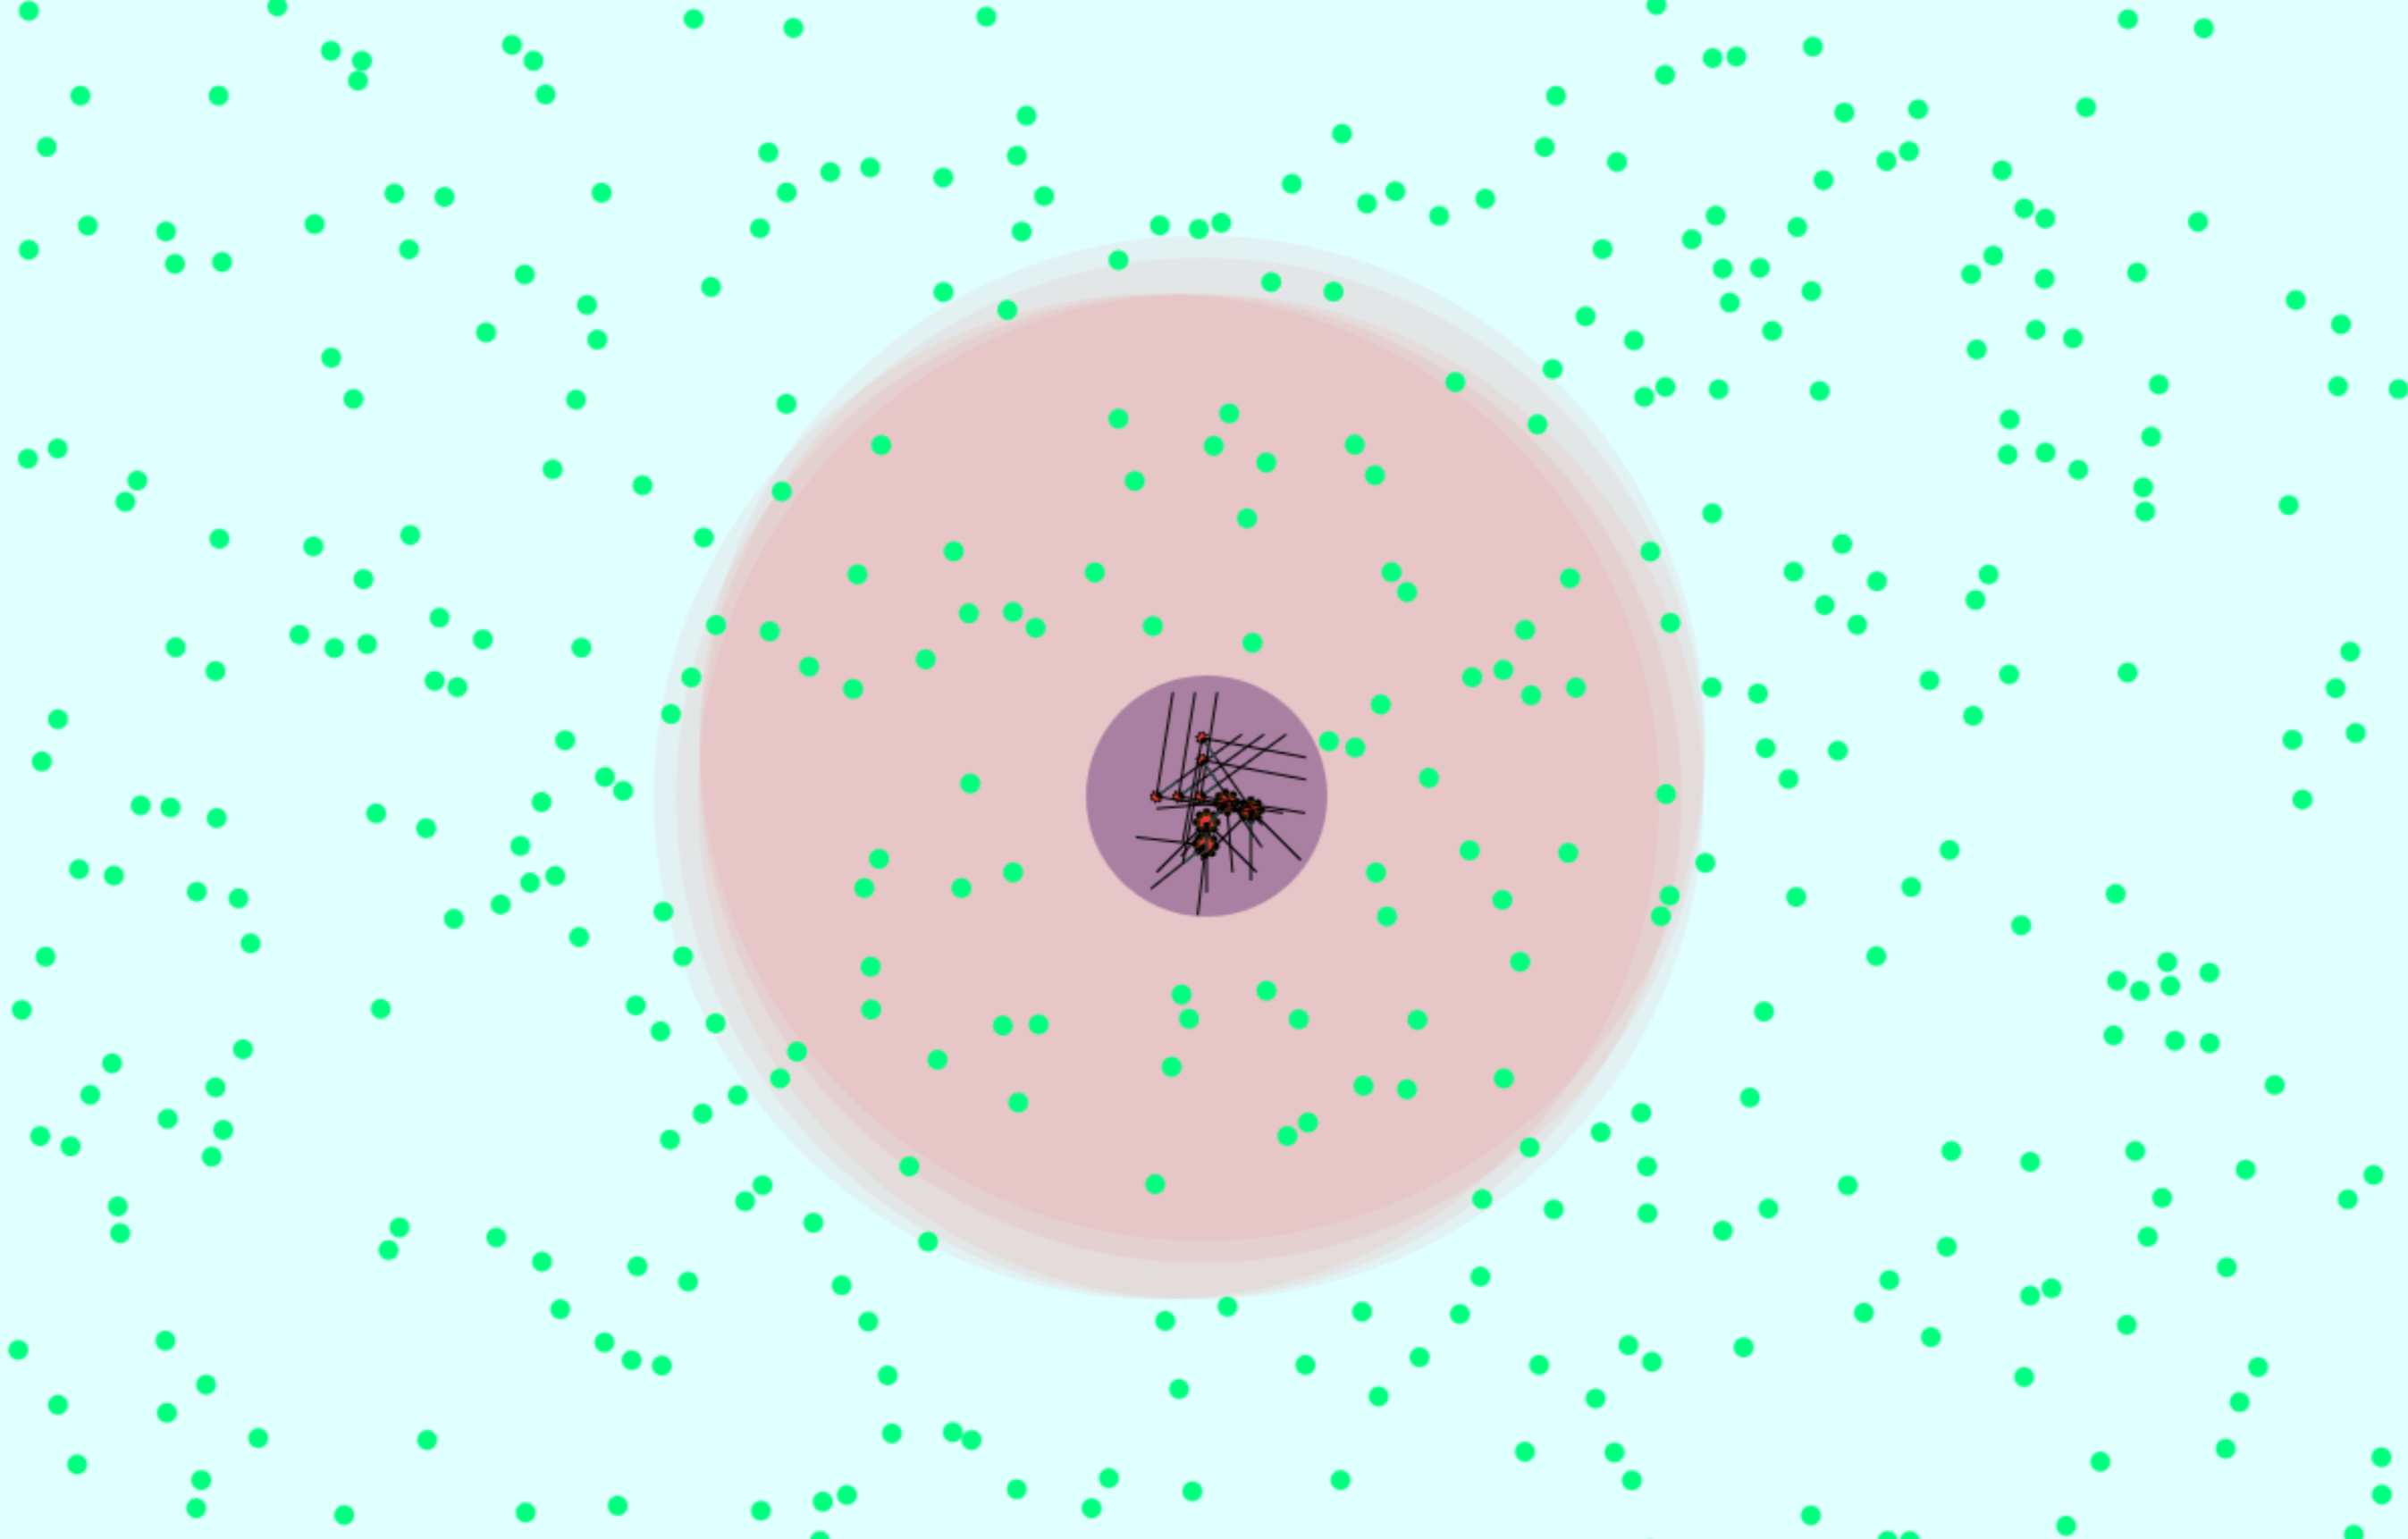
\includegraphics[width=\columnwidth]{../img/WoodMap/pictures/StartRandom.png}
	\caption{Příklad WoodScene mapy: start náhodného chování}
	\label{obr04:WoodSceneRandomStart}
\end{figure}
\par

\begin{figure}[p]\centering
	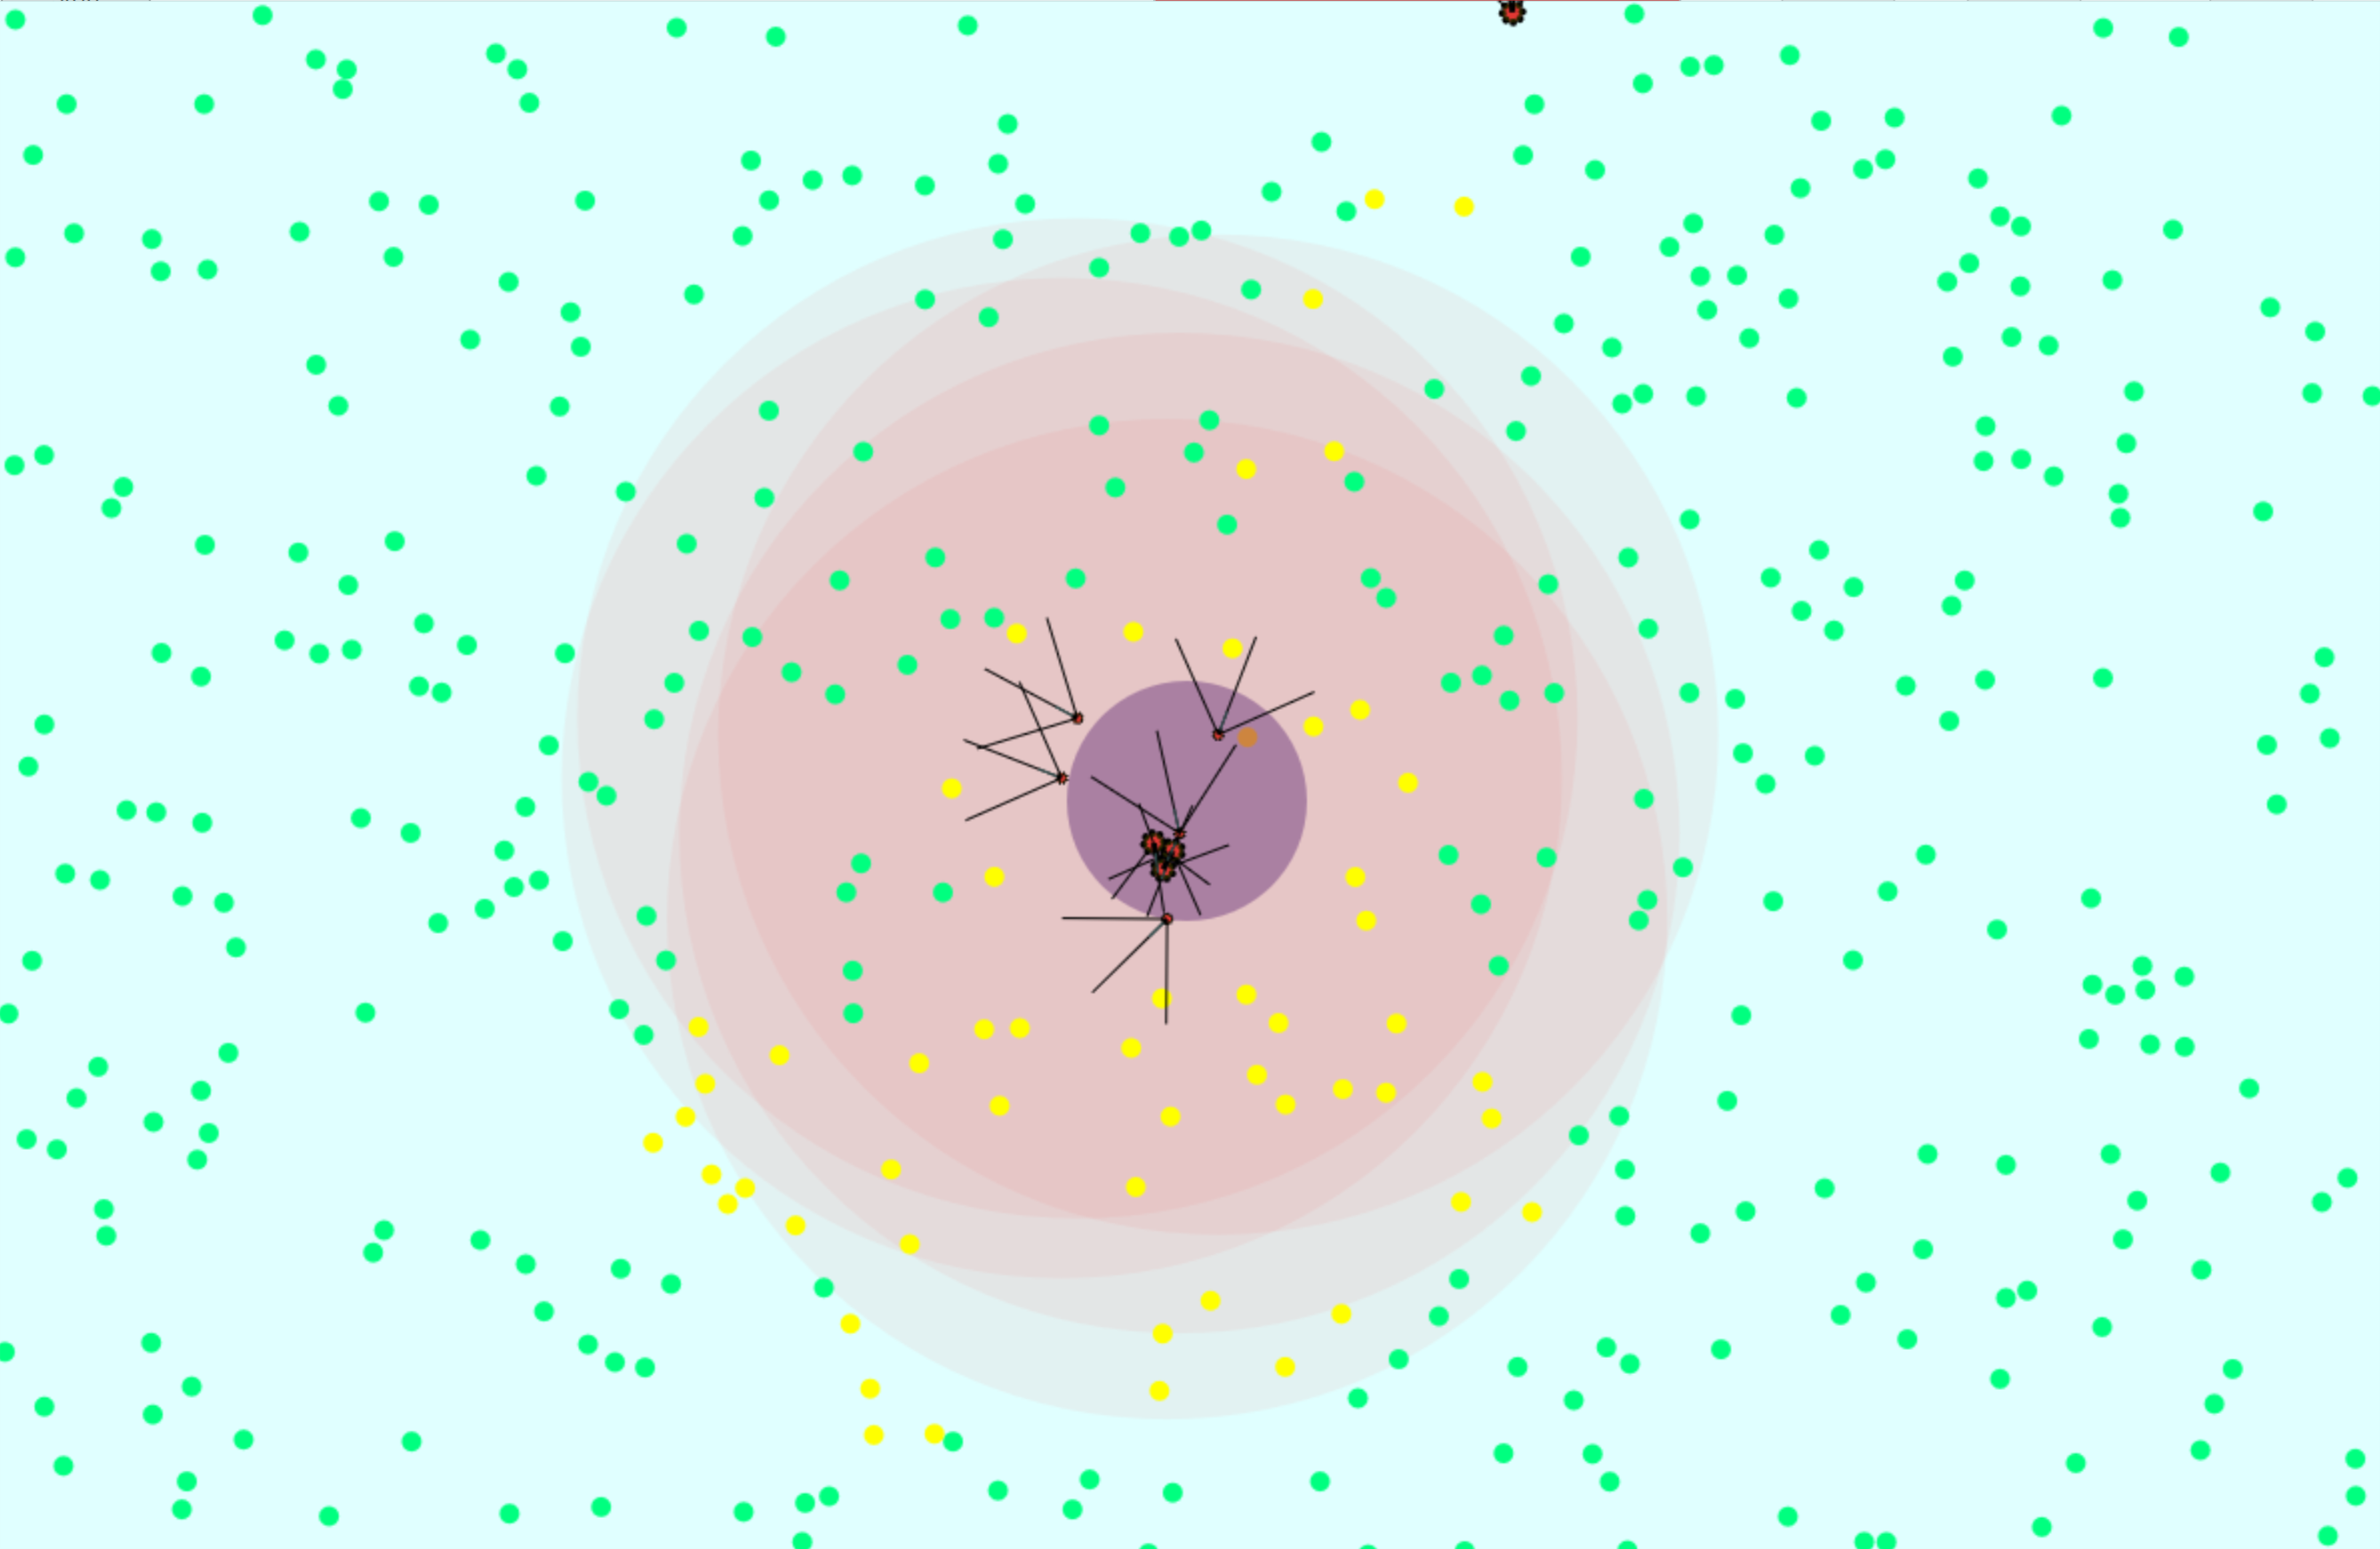
\includegraphics[width=\columnwidth]{../img/WoodMap/pictures/EndRandom.png}
	\caption{Příklad WoodScene mapy: po 9000 iteracích náhodného chování}
	\label{obr04:WoodSceneRandomEnd}
\end{figure}
\clearpage
\subsection{Roboti}
\subsubsection{Scout robot}
Jedná se o robota, který má na starosti průzkum mapy a kácení nalezených stromů. Pro komunikaci s ostatními roboty má možnost vysílat rádiový signál s hodnotou 0. Oproti Worker robotovi je menší, rychlejší, jeho senzory mají větší dosah, navíc proti němu disponuje type senzorem a refaktorem nalezených stromů. Type senzor představuje formu radaru, říká robotovi s jakou četností se vyskytují v dosahu senzoru. Refaktor reprezentuje techniku kácení mění strom na dřevo. 
\par 
\begin{table}[h]\centering
\begin{tabular}{l@{\hspace{1.0cm}}D{.}{,}{2.2}D{.}{,}{2.2}D{.}{,}{2.3}}
	\toprule
	\textbf{Scout Robot} \\
	\midrule
        Tvar: & Kruh & \\
        Poloměr: & 2.5 \\
        Název: & WoodCutterM \\
        Velikost kontejner: & 0\\
        \hline
        \textbf{Efektory} \\
        \midrule
        Motor: & Dvou kolečkový \\
        Maximální rychlost: & 3 \\
        Kód rádiového signálu: & 0 \\
        Poloměr signálu: & 200\\
        Refaktor: & Strom \Rightarrow Dřevo \\
        Dosah refaktoru: & 10\\
        Počet paměťových slotů: & 10 \\
        Obsah slotu: & float\\
        \hline 
        \textbf{Senzory} \\
        \midrule
        Počet line senzorů: &  3 \\
        Délka line senzorů: & 50\\
        Orientace line senzorů: & 0^\circ, 45^\circ, -45^\circ \\
        Poloměr type senzoru: & 50\\
        Poloměr rádiového přijímače: &  100 \\
        Počet touch senzorů: & 8 \\  
        Lokátor senzor\\ 
	\bottomrule
	\multicolumn{2}{l}{}
\end{tabular}
\caption{Wood - Scout robot popis}
\end{table}
\clearpage
\subsubsection{Worker robot}
Worker robot se stará o transport objektů na mapě. Ke komunikaci využívá signálů s kódem 1. Sebrané objekty ukládá do kontejneru, kam se vejde 5 entit. Zvedání a pokládání probíhá skrze efektor Picker. 
\par 
\begin{table}[h]\centering
	\begin{tabular}{l@{\hspace{1.0cm}}D{.}{,}{2.2}D{.}{,}{2.2}D{.}{,}{2.3}}
			\toprule
			\textbf{Worker Robot} \\
			\midrule
                Tvar: & Kruh\\
                Poloměr: & 5\\
                Název: & WoodWorkerM \\
                Velikost kontejner: & 5\\
                \hline
                \textbf{Efektory} \\
                \midrule
                Motor: & Dvou kolečkový \\
                Maximální rychlost: & 2 \\
                Kód rádiového signálu: & 0\\
                Poloměr signálu: & 200\\
                Dosah pickeru: & 10\\
                Počet paměťových slotů: &10 \\
                Obsah slotu: & float\\
                \hline 
                \textbf{Senzory} \\
                \midrule
                Počet line senzorů: &  3\\
                Délka line senzorů: & 30\\
                Orientace line senzorů: & 0^\circ, 45^\circ, -45^\circ\\
                Poloměr rádiového přijímače: & 100 \\
                Počet touch senzorů: & 8 \\  
                Lokátorový senzor\\ 
	\bottomrule
\multicolumn{2}{l}{}
\end{tabular}
\caption{Wood - Worker robot popis }
\end{table}
\clearpage
\subsection{Vyhodnocování Fitness}
Fitness funkce pro ohodnocení WoodScene scénáře probíhá vždy až na konci simulace. I když se úspěšnost v podúkolech  vždy posuzuje jinak, celou fitness funkci lze shrnout do následujícího cílů. Roboti jsou odměňováni za: 
\begin{enumerate}
        \item nalezené stromy = stromy o které zavadil line senzor 
        \item pokácené stromy = stromy, které refaktor změnil 
        \item sebrané dřevo = zpracované dřevo, které mají roboti uvnitř kontejnerů 
        \item uskladněné dřevo = dřevo, které dovezli na vyznačené místo 
\end{enumerate}
Trestáni za:
\begin{enumerate}
	\item kolize = počet pokusů o pohyb při kterém by došlo ke kolizi 
\end{enumerate}

\subsection{Podúkoly} 
Pro oba použité algoritmy jsem používal stejné úlohy pro naučení robotů postupně těžších a těžších cílů. Hlavně také, abych mohl porovnat oba evoluční algoritmy.  
\begin{enumerate}
        \item vygenerování robotů = Na začátku je vygenerováno chování robotů naprosto náhodně. Pro každého robota, je vygenerována náhodná jednovrstvá neuronová síť. 
        \item učení chůze = Pro oba roboty je velmi důležité, aby se pohybovali bez kolizí po celé mapě a objevovali, co největší prostor. Roboti jsou vyvíjeni odděleně a fitness se soustředí na počet kolizí (záporným ohodnocením) a na nalezené stromy (kladným ohodnocením).
        \item těžba stromů = Scout roboty, kteří se už obstojně po mapě pohybují, je třeba naučit kácet stromy. Proto dalším  cílem ve fitness funkci je počet pokácených stromů. Nicméně stále také na počet stromů nalezených. 
        \item převoz dřeva = Správně pohybující chceme naučit sbírat vytěžené dřevo. Fitness hodnotí počet sebraného dřeva, případně i uskladněné dřevo. Na těchto mapách jsou už na začátku připraveny pouze entity zpracovaného dřeva.
        \item kooperace = V posledním experimentu, se hodnotí pouze sebrané a uskladněné dřevo. A evolvují se oba druhy robotů současně. 
\end{enumerate}

\newpage
	\subsubsection{Scout chůze - nastavení experimentu}
	\begin{table}[h]\centering
		\begin{tabular}{l@{\hspace{1.5cm}}D{.}{,}{3.2}D{.}{,}{1.2}D{.}{,}{2.3}}
			\toprule
			& \mc{} & \mc{}\\
			\pulrad{\textbf{Vlastnost:}} & \mc{\pulrad{\textbf{Hodnota:}}}\\
			\midrule
			Roboti:     & Scout-5 \\
			Počet generací: & 1000\\
			Počet iterací map & 1000\\
			Velikost generace(DE) & 200\\
			Počet jedinců(ES) & 10\\
			Počet mutovaný potomků(ES)&20\\
			Elitismus(ES)& Ano\\
			Elitismus(DE)& Ne \\
			\bottomrule
			\multicolumn{2}{l}{}
		\end{tabular}
		\begin{tabular}{l@{\hspace{1.5cm}}D{.}{,}{3.2}D{.}{,}{1.2}D{.}{,}{2.3}}
			\toprule
			& \mc{} & \mc{}\\
			\pulrad{\textbf{Vlastnost:}} & \mc{\pulrad{\textbf{Hodnota:}}}\\
			\midrule
			Hodnota nalezeného stromu &  10 \\
			Ostatní hodnoty: & 0\\
			Počet stromů: & 300\\
			Počet už pokácených stromů & 100\\
			\bottomrule
			\multicolumn{2}{l}{}
		\end{tabular}
		\caption{Scout chůze - nastavení experimentu}\label{tab04:ScoutWalk}
	\end{table}
	\improvement{Roztáhnout osy, aby graf nepřetékal}
	\begin{figure}[t]\centering
		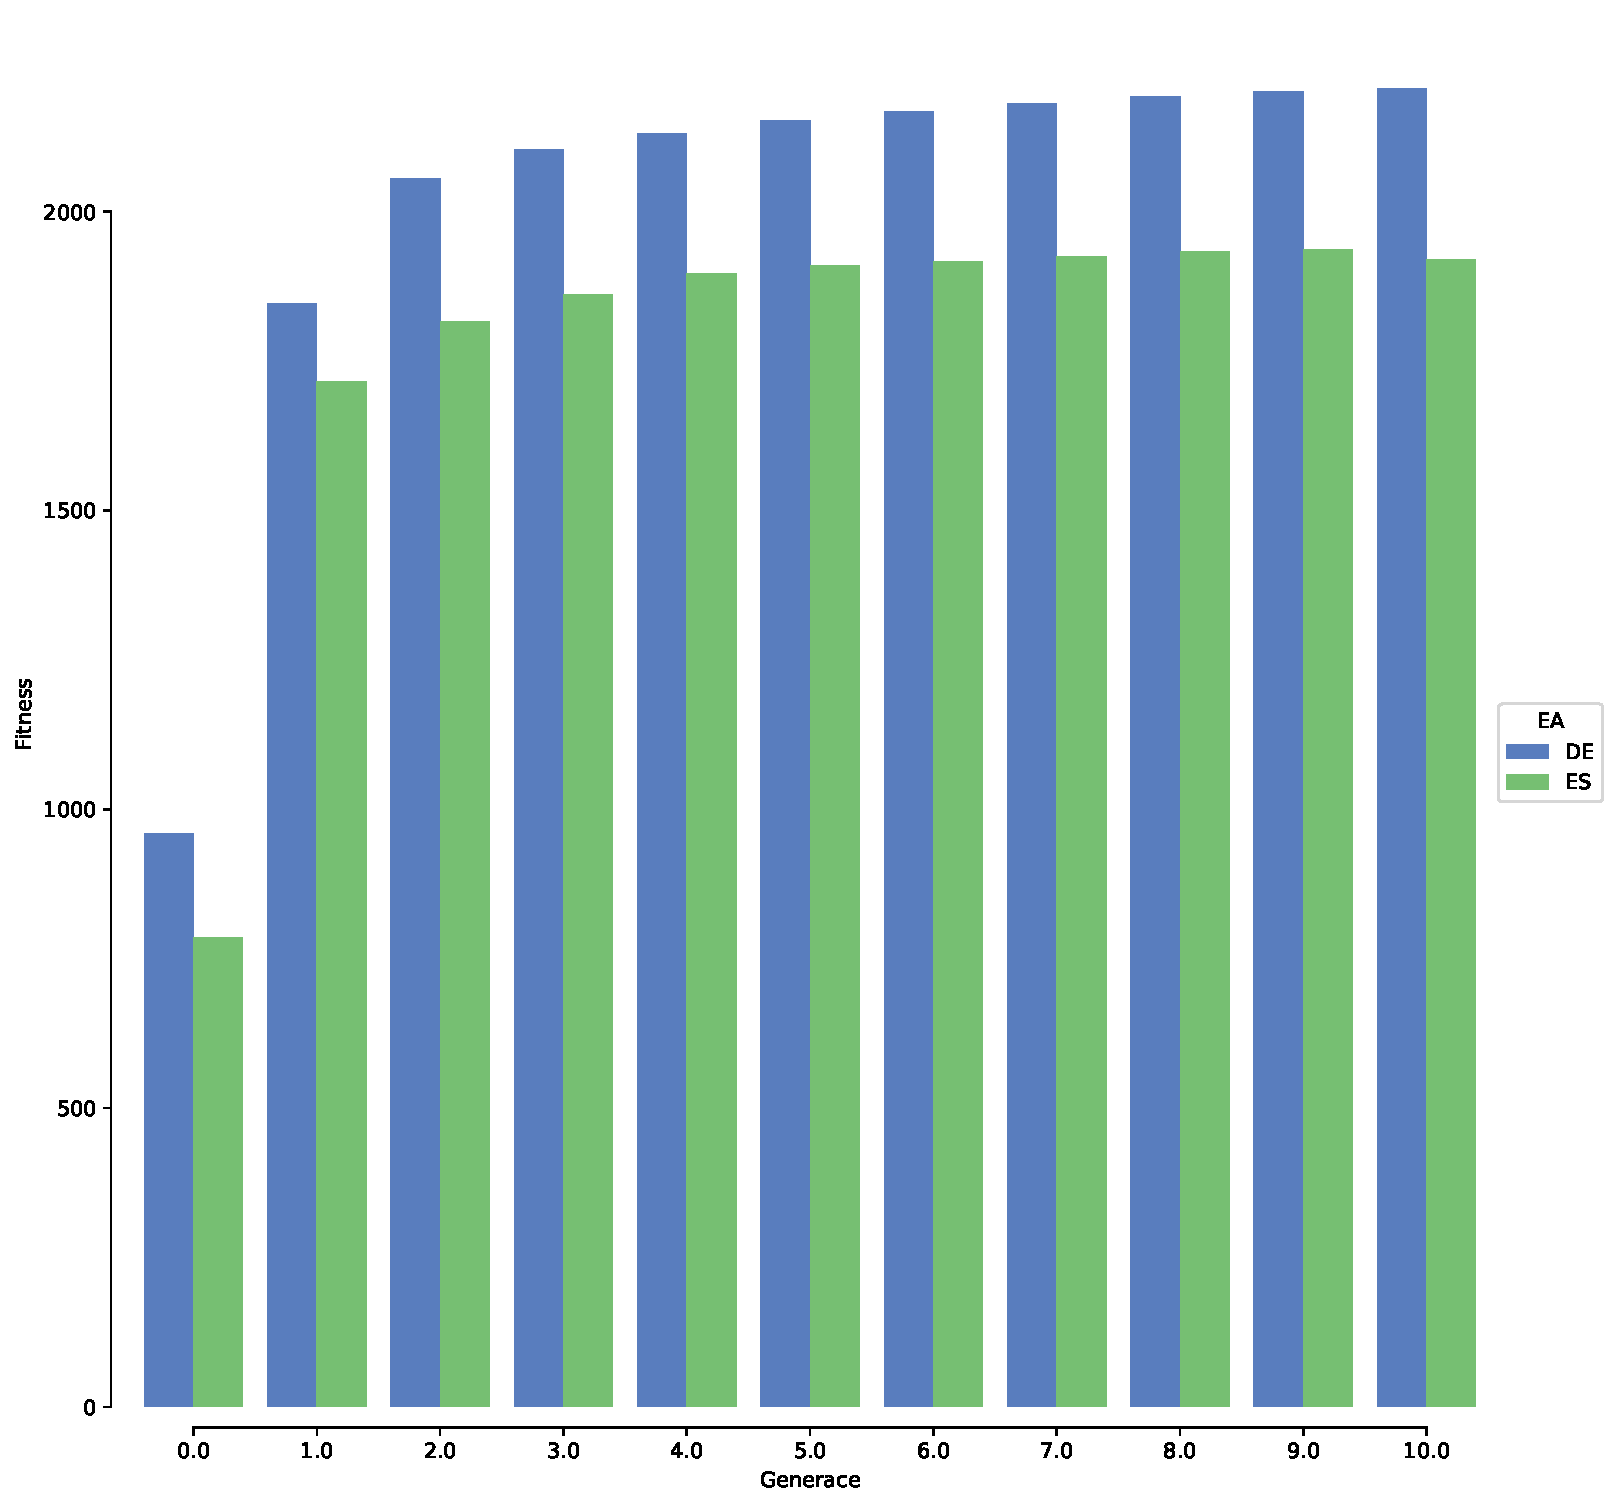
\includegraphics[width=\columnwidth]{../img/WoodMap/DEvsES/WCuttorWalkMem}
		\caption{ Scout chůze - porovnání průměrné fitness ES a DE}
		\label{obr04:WalkESvsDE}
	\end{figure}
	\redo{Opravit obrázky - rozsahy a popisy}
	\begin{figure}[p]
		\centering
		\begin{subfigure}{.5\textwidth}
			\centering
			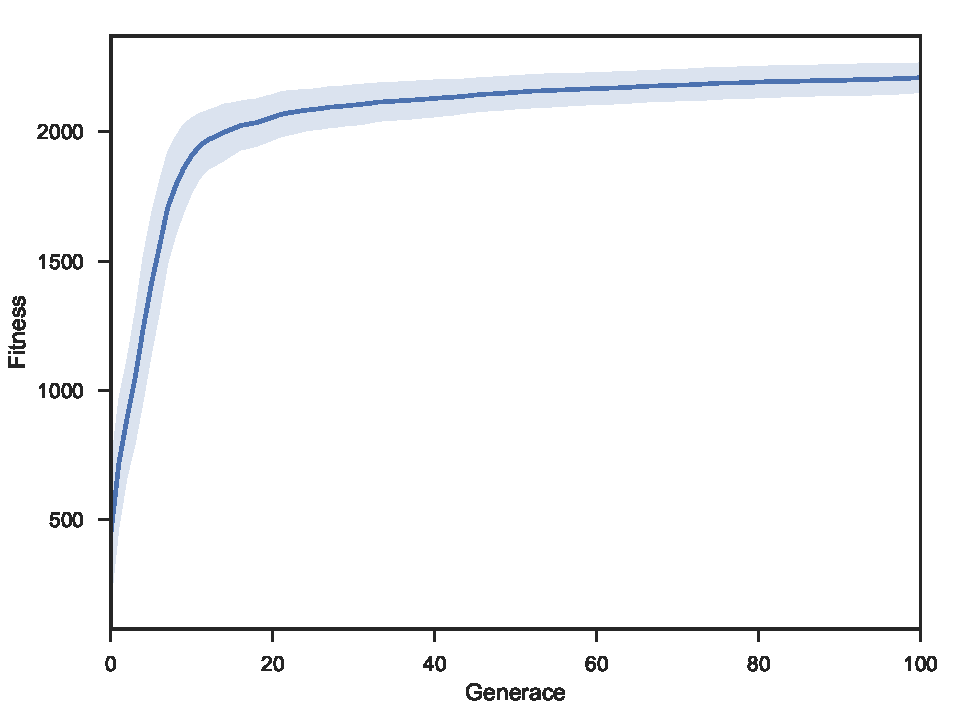
\includegraphics[width=\linewidth]{../img/WoodMap/DE/WCuttorWalkMem}
			\caption{DE}
			\label{obr04:WalkDE}
		\end{subfigure}%
		\begin{subfigure}{.5\textwidth}
			\centering
			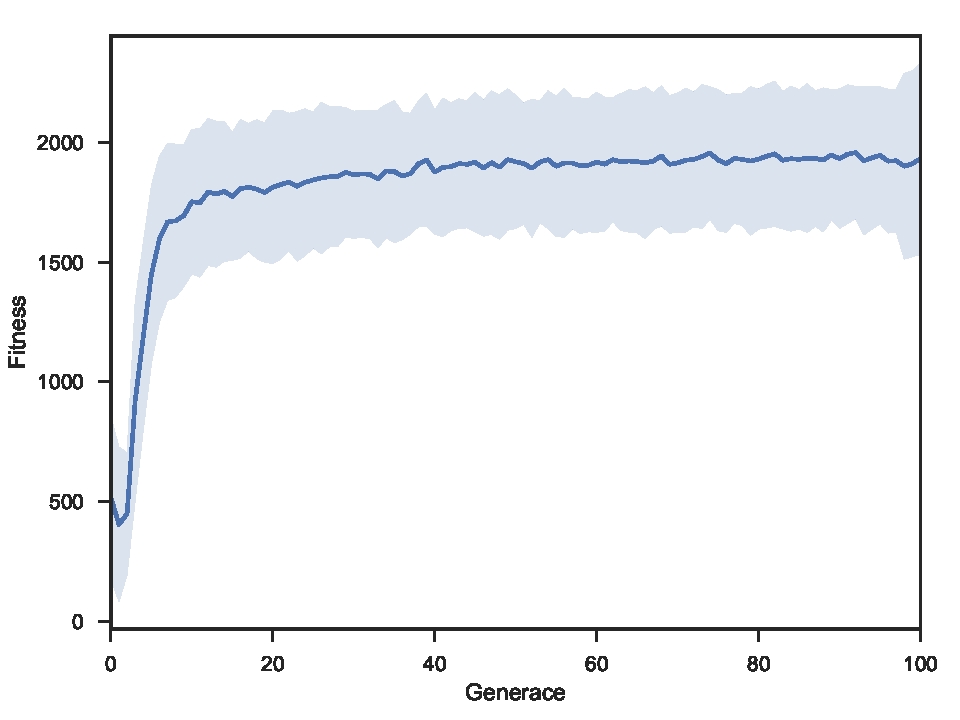
\includegraphics[width=\linewidth]{../img/WoodMap/ES/WoodWalkES}
			\caption{ES}
			\label{obr04:WalkES}
		\end{subfigure}
		\caption{Scout chůze - průběh fitness }
		\label{obr04:Walk}
	\end{figure}
	\clearpage
	
	\subsubsection{Worker chůze - nastavení experimentu}
	\begin{table}[h]\centering
		\begin{tabular}{l@{\hspace{1.5cm}}D{.}{,}{3.2}D{.}{,}{1.2}D{.}{,}{2.3}}
			\toprule
			& \mc{} & \mc{}\\
			\pulrad{\textbf{Vlastnost:}} & \mc{\pulrad{\textbf{Hodnota:}}}\\
			\midrule
			Roboti:     & Worker-4 \\
			Počet generací: & 1000\\
			Počet iterací map & 1000\\
			Velikost generace(DE) & 200\\
			Počet jedinců(ES) & 10\\
			Počet mutovaný potomků(ES)&20\\
			Elitismus(ES)& Ano\\
			Elitismus(DE)& Ne \\
			\bottomrule
			\multicolumn{2}{l}{}
		\end{tabular}
		\begin{tabular}{l@{\hspace{1.5cm}}D{.}{,}{3.2}D{.}{,}{1.2}D{.}{,}{2.3}}
			\toprule
			& \mc{} & \mc{}\\
			\pulrad{\textbf{Vlastnost:}} & \mc{\pulrad{\textbf{Hodnota:}}}\\
			\midrule
			Hodnota nalezeného pokáceného stromu &  100 \\
			Ostatní hodnoty: & 0\\
			Počet stromů: & 200\\
			Počet už pokácených stromů & 200\\
			\bottomrule
			\multicolumn{2}{l}{}
		\end{tabular}
		\caption{Worker chůze - nastavení experimentu}
		\label{tab04:WorkerWalk}
	\end{table}
	
	\begin{figure}[t]\centering
		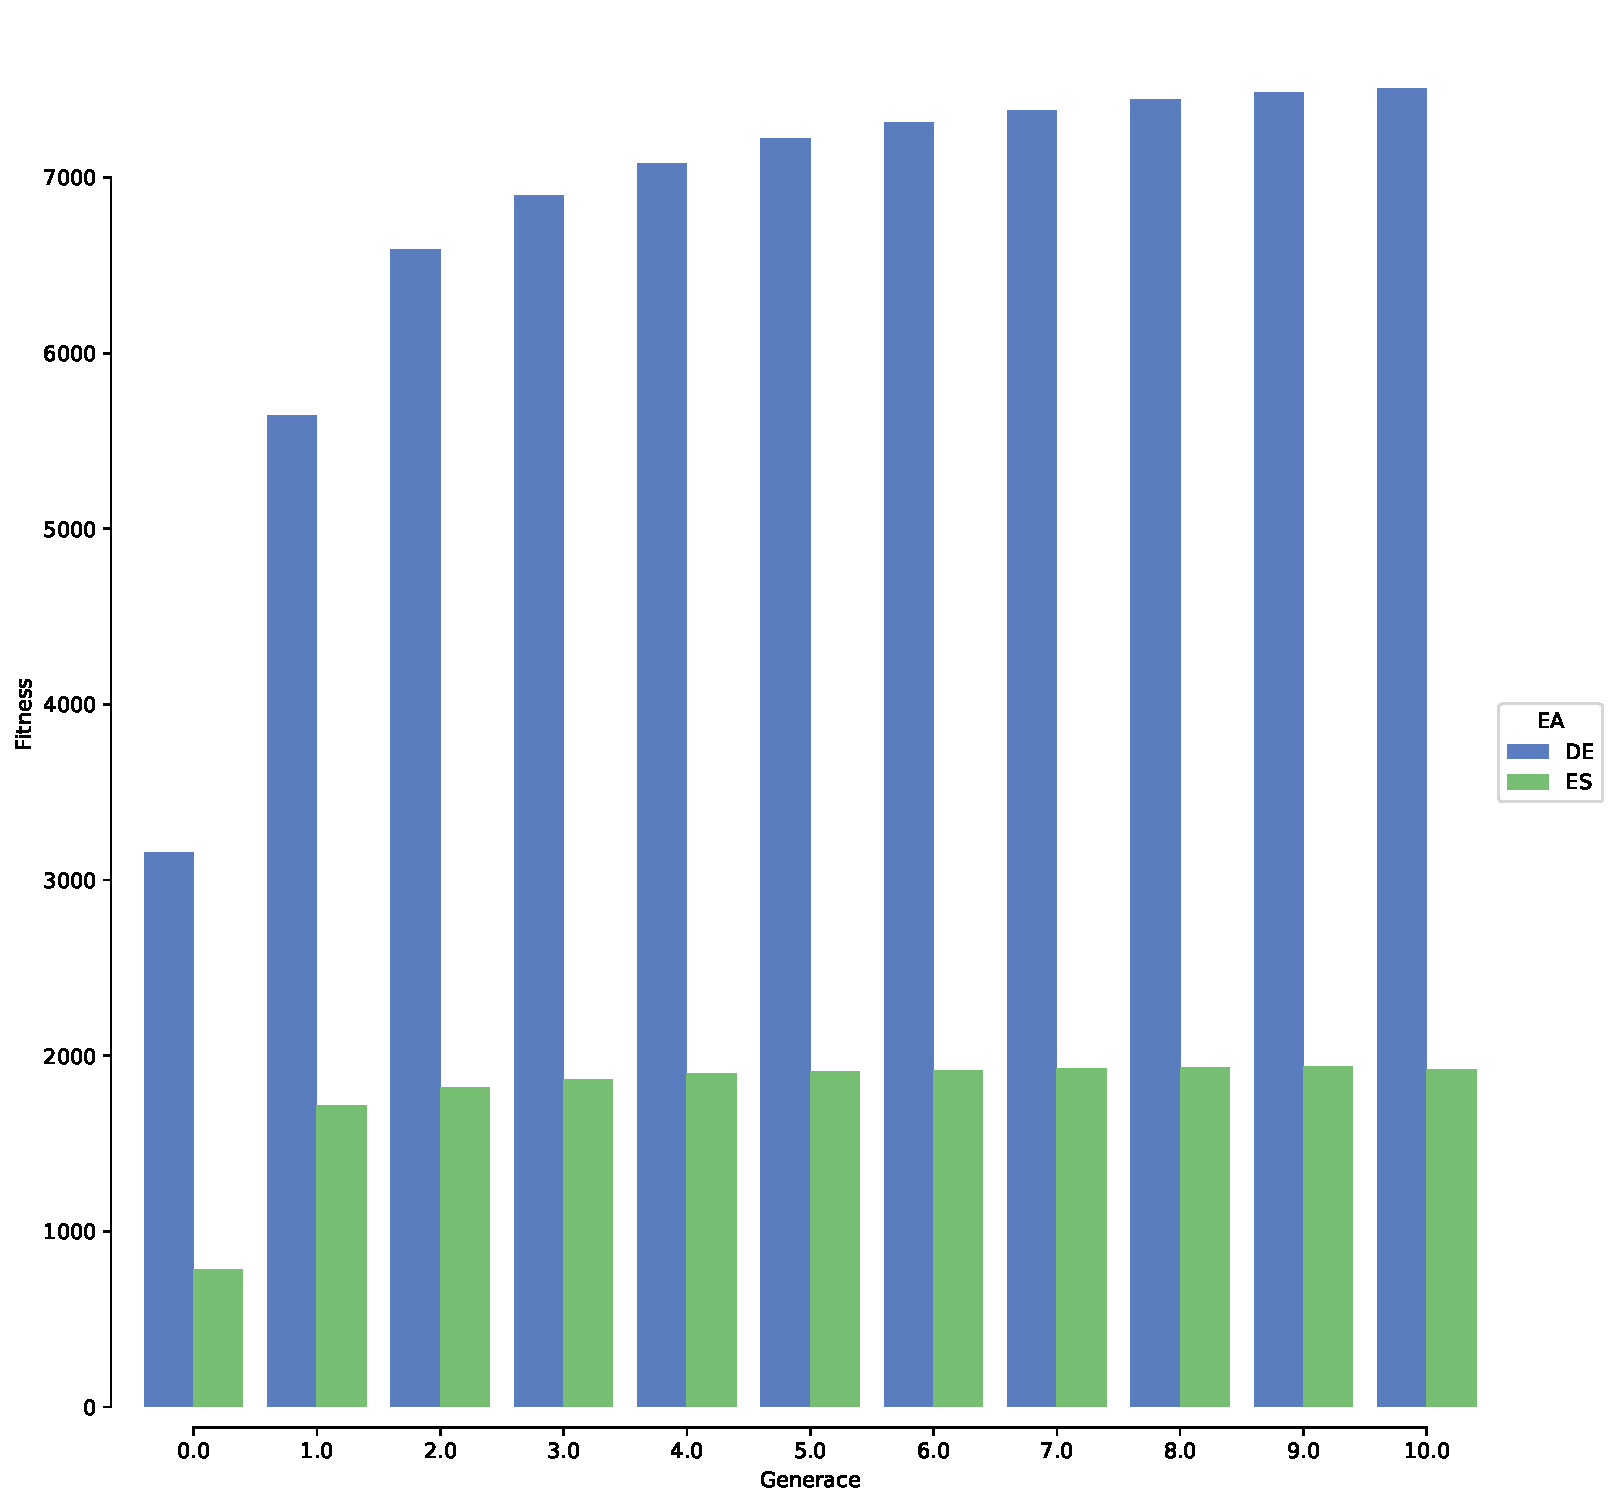
\includegraphics[width=\columnwidth]{../img/WoodMap/DEvsES/WorkerWalkMem}
		\caption{Worker chůze - porovnání průměrné fitness ES a DE}
		\label{obr04:WWalkESvsDE}
	\end{figure}
	\redo{Opravit rozsahy a rozlišení}
	\begin{figure}[p]
		\centering
		\begin{subfigure}{.5\textwidth}
			\centering
			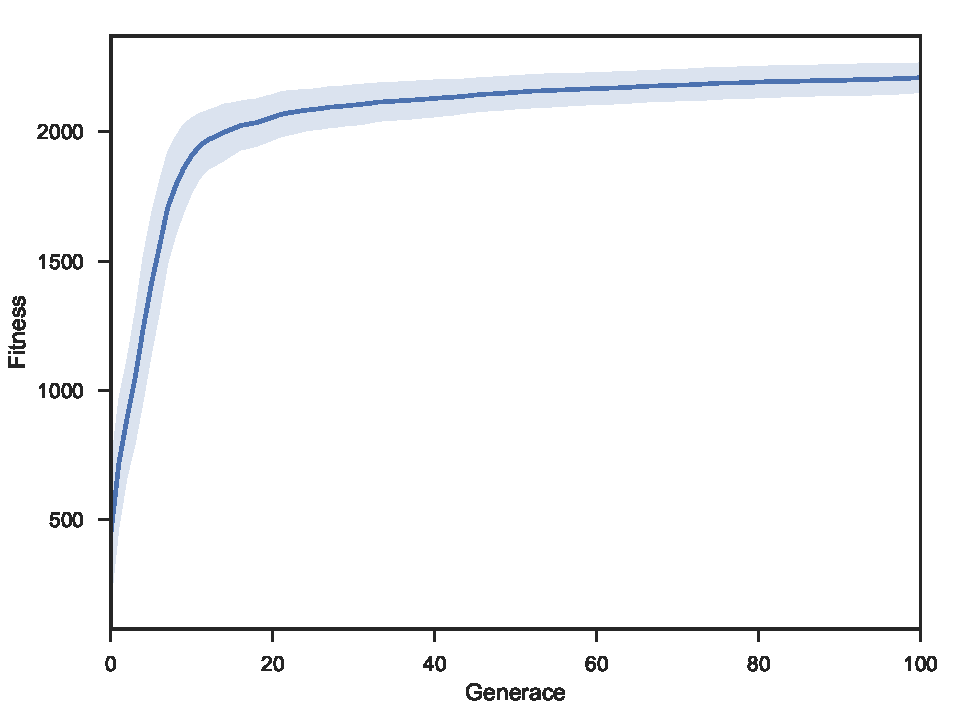
\includegraphics[width=\linewidth]{../img/WoodMap/DE/WCuttorWalkMem}
			\caption{DE}
			\label{obr04:WWalkDE}
		\end{subfigure}%
		\begin{subfigure}{.5\textwidth}
			\centering
			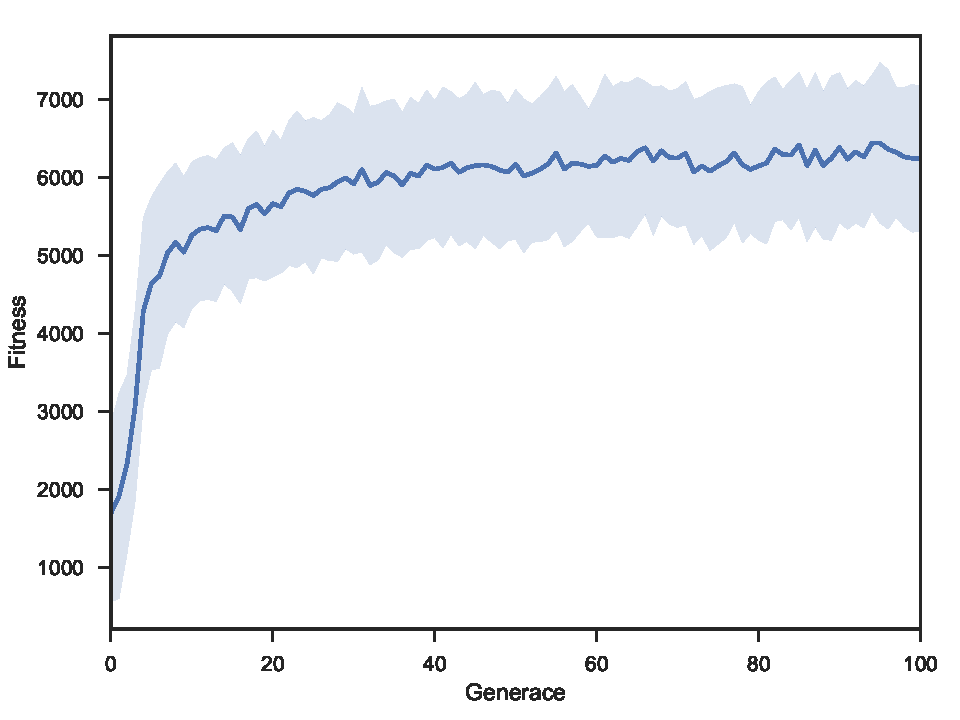
\includegraphics[width=\linewidth]{../img/WoodMap/ES/WoodWWalkES}
			\caption{ES}
			\label{obr04:WWalkES}
		\end{subfigure}
		\caption{Worker chůze - průběh fitness v rámci generací}
		\label{obr04:WWalk}
	\end{figure}
	\clearpage 
	
	
	
	\subsubsection{Scout kácení - nastavení experimentu}
	\begin{table}[h]\centering
		\begin{tabular}{l@{\hspace{1.5cm}}D{.}{,}{3.2}D{.}{,}{1.2}D{.}{,}{2.3}}
			\toprule
			& \mc{} & \mc{}\\
			\pulrad{\textbf{Vlastnost:}} & \mc{\pulrad{\textbf{Hodnota:}}}\\
			\midrule
			Roboti:     & Scout-5 \\
			Počet generací: & 1500\\
			Počet iterací map & 1000\\
			Velikost generace(DE) & 200\\
			Počet jedinců(ES) & 10\\
			Počet mutovaný potomků(ES)&20\\
			Elitismus(ES)& Ano\\
			Elitismus(DE)& Ne \\
			\bottomrule
			\multicolumn{2}{l}{}
		\end{tabular}
		\begin{tabular}{l@{\hspace{1.5cm}}D{.}{,}{3.2}D{.}{,}{1.2}D{.}{,}{2.3}}
			\toprule
			& \mc{} & \mc{}\\
			\pulrad{\textbf{Vlastnost:}} & \mc{\pulrad{\textbf{Hodnota:}}}\\
			\midrule
			Hodnota nalezeného stromu &  1000\\
			Hodnota pokáceného stromu & 10000\\
			Hodnota kolize & -1\\
			Ostatní hodnoty: & 0\\
			Počet stromů: & 400\\
			Počet už pokácených stromů & 0\\
			\bottomrule
			\multicolumn{2}{l}{}
		\end{tabular}
		\caption{Scout kácení - nastavení experimentu}
	\end{table}
	
	\begin{figure}[t]\centering
		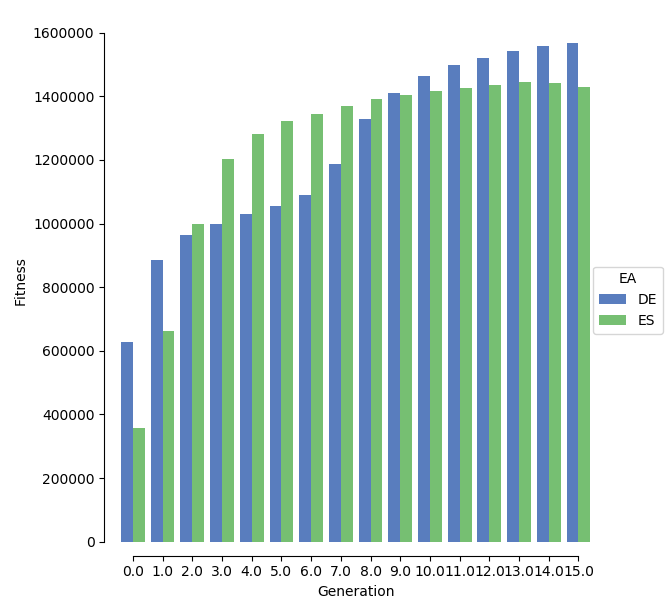
\includegraphics[width=\columnwidth]{../img/WoodMap/DEvsES/WCuttorCutMem}
		\caption{Scout kácení - porovnání průměrné fitness ES a DE}
		\label{obr04:CutESvsDE}
	\end{figure}
	\redo{Opravit obrázky}
	\begin{figure}[p]
		\centering
		\begin{subfigure}{.5\textwidth}
			\centering
			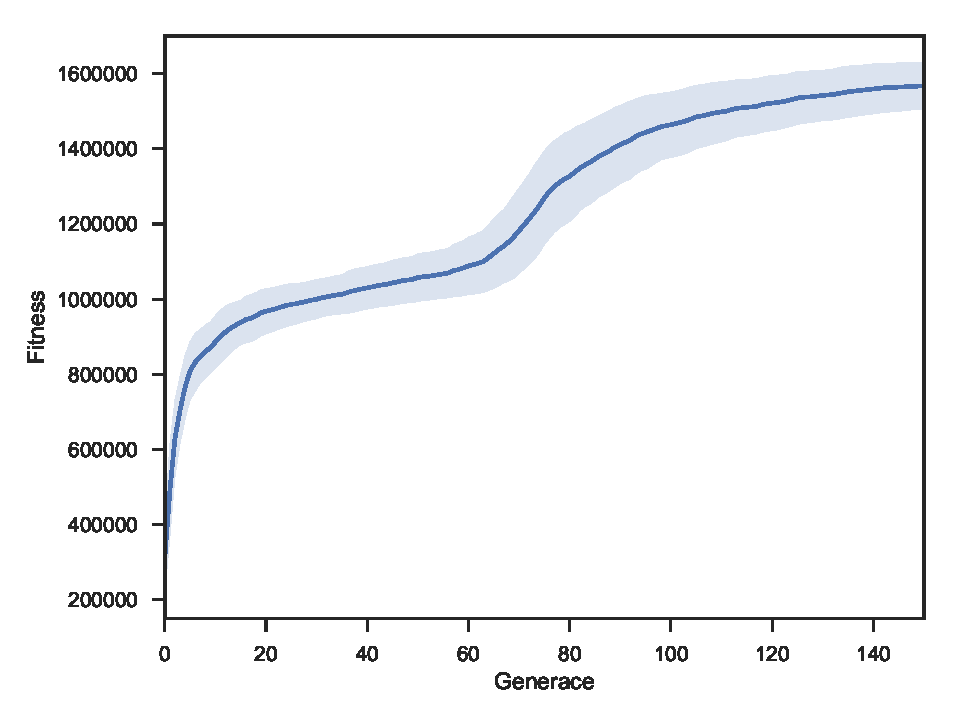
\includegraphics[width=\linewidth]{../img/WoodMap/DE/WCuttorCutMem}
			\caption{DE}
			\label{obr04:CutDE}
		\end{subfigure}%
		\begin{subfigure}{.5\textwidth}
			\centering
			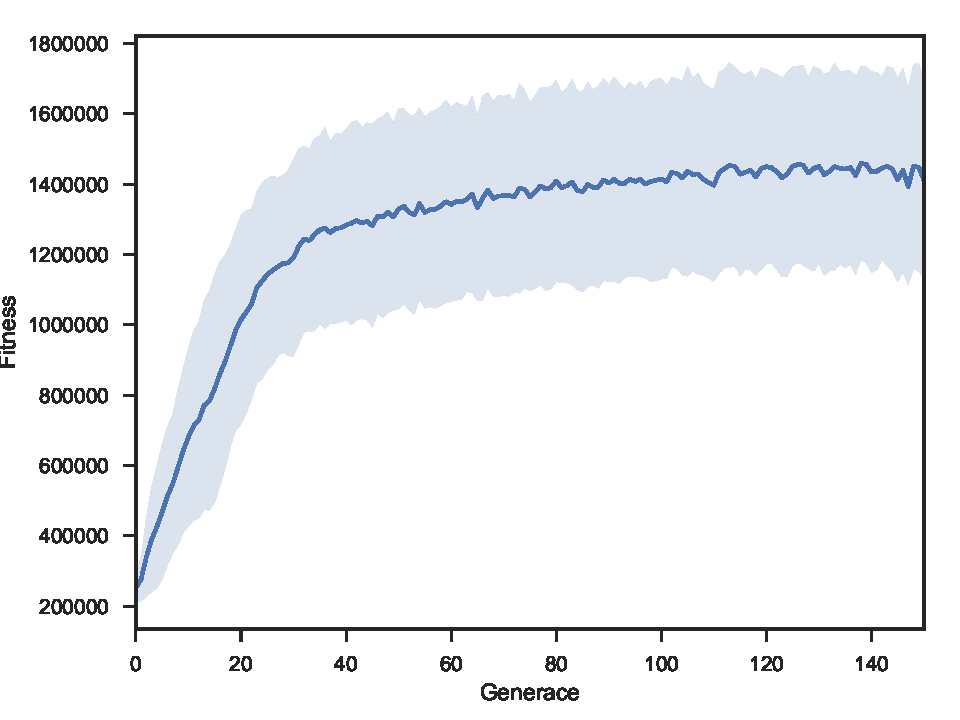
\includegraphics[width=\linewidth]{../img/WoodMap/ES/WoodCutES}
			\caption{ES}
			\label{obr04:CutES}
		\end{subfigure}
		\caption{Scout kácení - průběh fitness v rámci generací}
		\label{obr04:Cut}
	\end{figure}
	\clearpage
	
	\subsubsection{Worker sbírání - nastavení experimentu}
	\begin{table}[h]\centering
		\begin{tabular}{l@{\hspace{1.5cm}}D{.}{,}{3.2}D{.}{,}{1.2}D{.}{,}{2.3}}
			\toprule
			& \mc{} & \mc{}\\
			\pulrad{\textbf{Vlastnost:}} & \mc{\pulrad{\textbf{Hodnota:}}}\\
			\midrule
			Roboti:     & Worker-4 \\
			Počet generací: & 2000\\
			Počet iterací map & 1000\\
			Velikost generace(DE) & 200\\
			Počet jedinců(ES) & 10\\
			Počet mutovaný potomků(ES)&20\\
			Elitismus(ES)& Ano\\
			Elitismus(DE)& Ne \\
			\bottomrule
			\multicolumn{2}{l}{ }
		\end{tabular}
		\par 
		\begin{tabular}{l@{\hspace{1.5cm}}D{.}{,}{3.2}D{.}{,}{1.2}D{.}{,}{2.3}}
			\toprule
			& \mc{} & \mc{}\\
			\pulrad{\textbf{Vlastnost:}} & \mc{\pulrad{\textbf{Hodnota:}}}\\
			\midrule
			Hodnota nalezeného pokáceného stromu &  100 \\
			Hodnota uloženého dřeva & 1010\\
			Hodnota dřeva v kontejneru & 1000\\
			Hodnota jiné entity v kontejneru & -100\\
			Hodnota kolize & -1\\
			Ostatní hodnoty: & 0\\
			Počet stromů: & 200\\
			Počet už pokácených stromů & 200\\
			\bottomrule
			\multicolumn{2}{l}{}
		\end{tabular}
		\caption{Worker sbírání - nastavení experimentu}
	\end{table}
	\begin{figure}[t]\centering       
		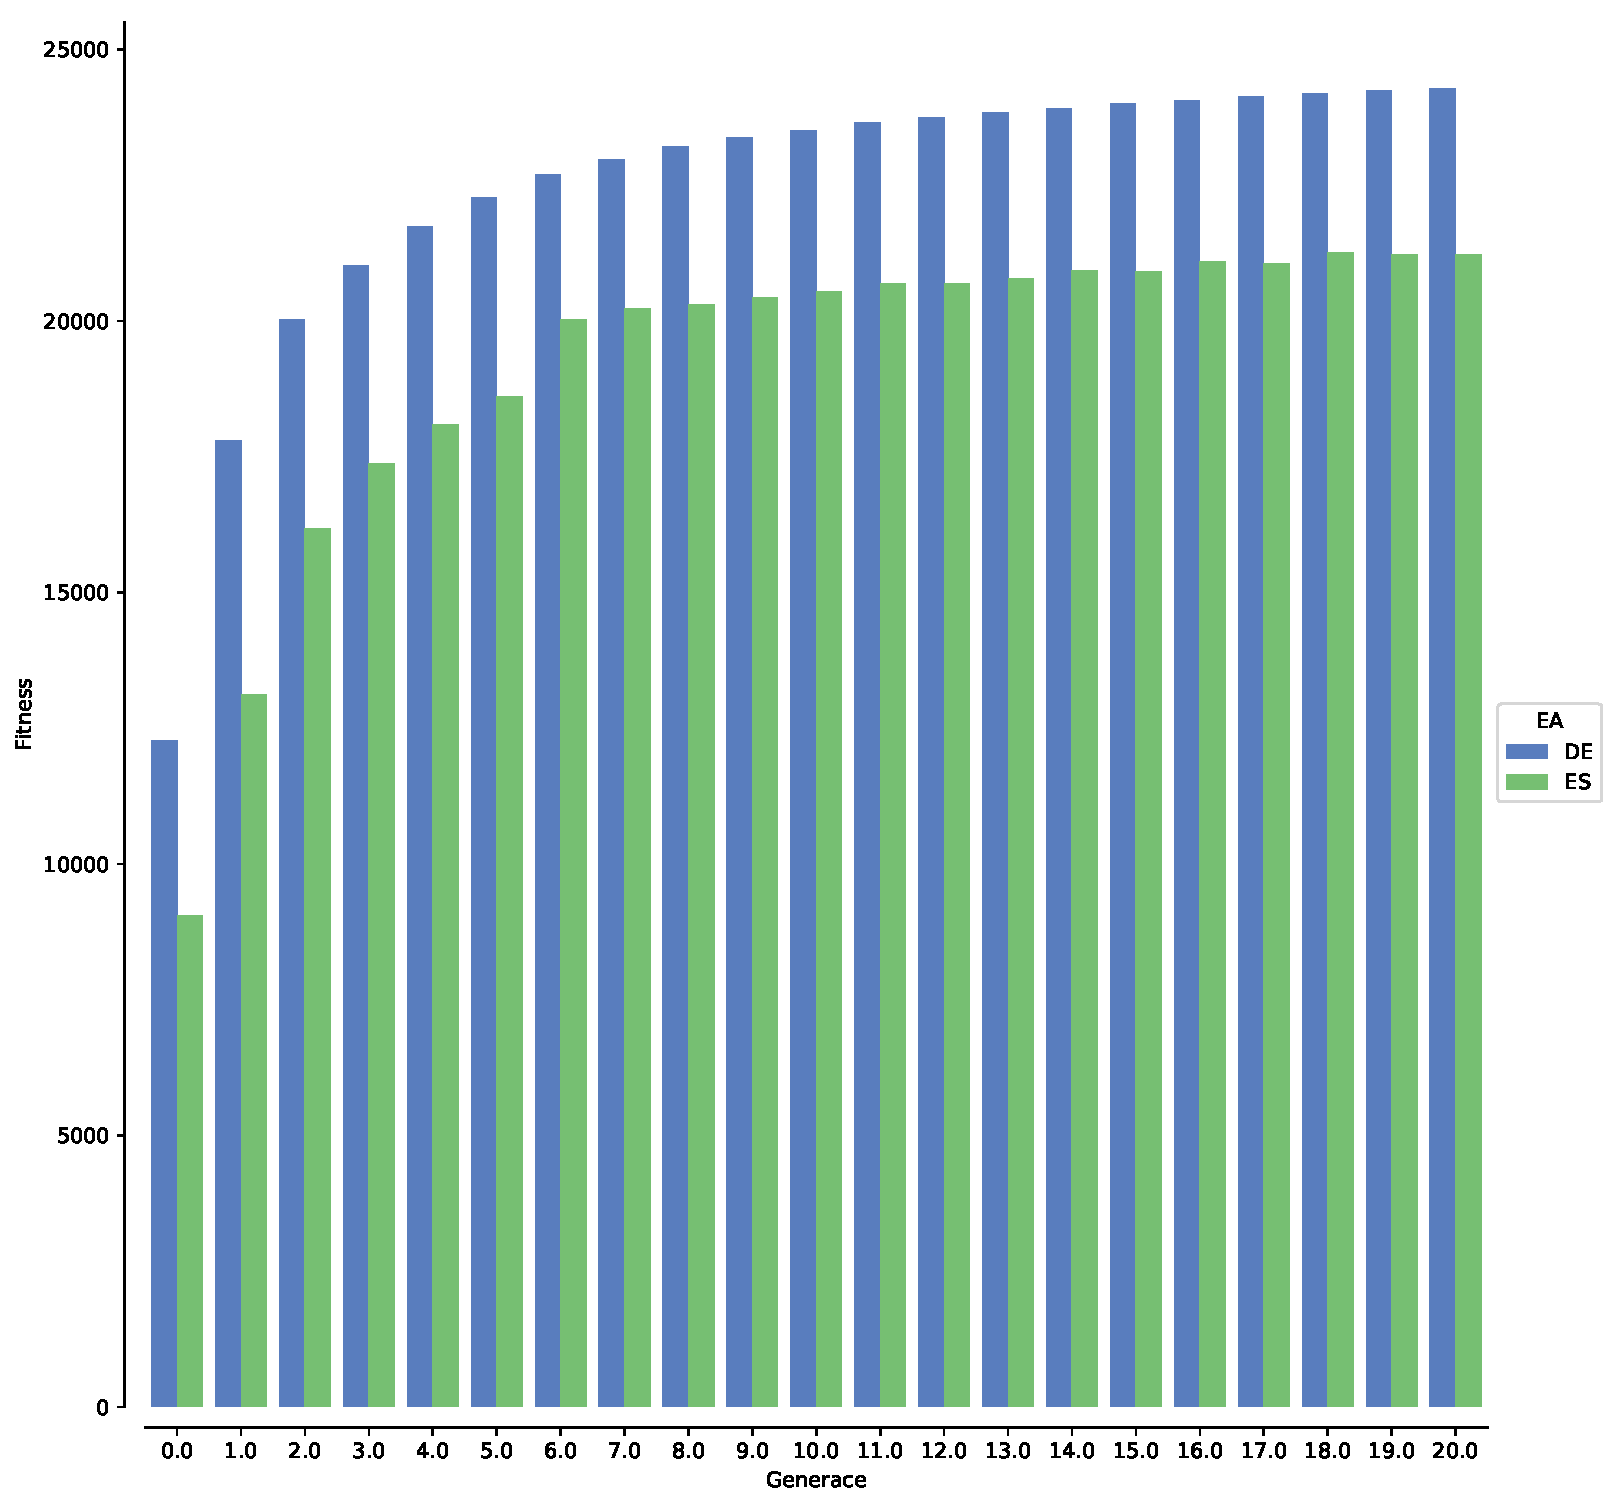
\includegraphics[width=\columnwidth]{../img/WoodMap/DEvsES/WorkerPickUpMem}
		\caption{ Worker sbírání - porovnání průměrné fitness ES a DE}
		\label{obr04:PickupESvsDE}
	\end{figure}
	\redo{Opravit obrázky
	}\begin{figure}[p]
		\centering
		\begin{subfigure}{.5\textwidth}
			\centering
			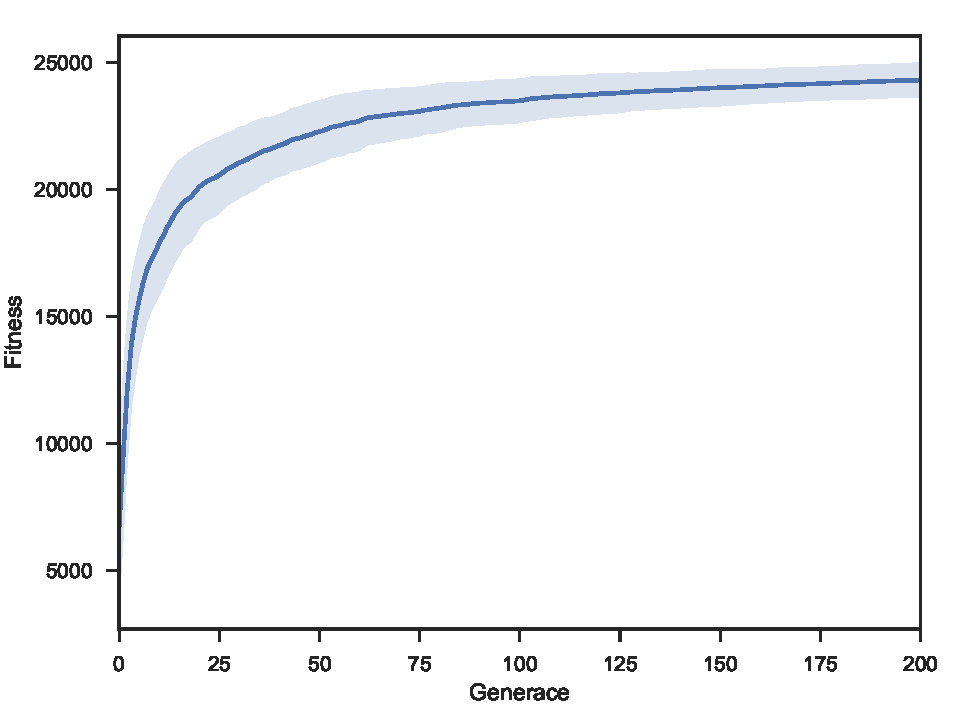
\includegraphics[width=\linewidth]{../img/WoodMap/DE/WorkerPickUpMem}
			\caption{DE}
			\label{obr04:PickupDE}
		\end{subfigure}%
		\begin{subfigure}{.5\textwidth}
			\centering
			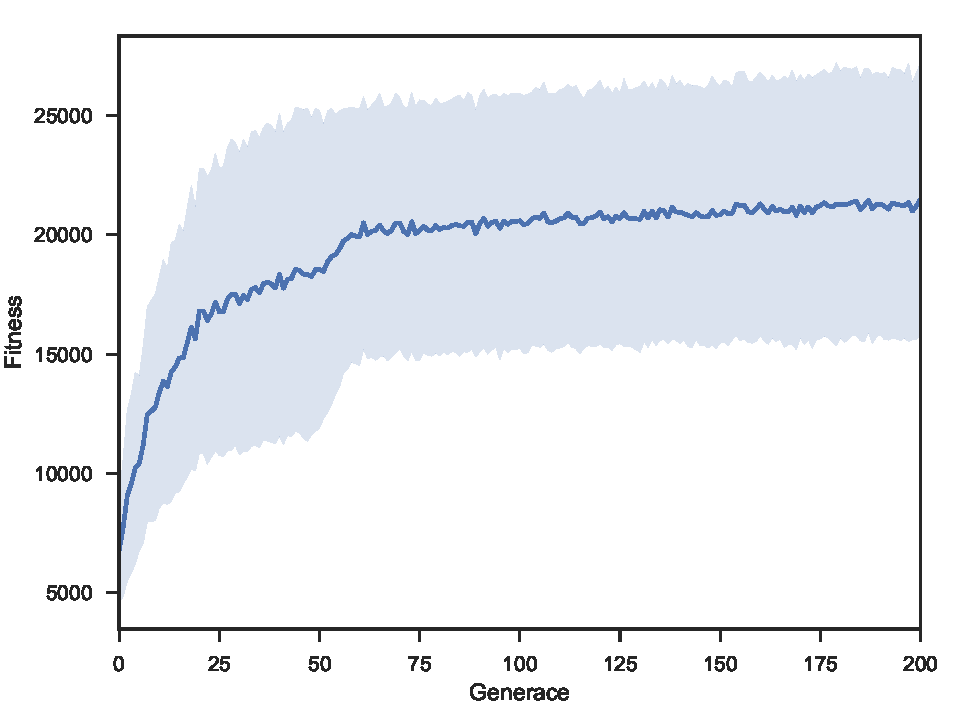
\includegraphics[width=\linewidth]{../img/WoodMap/ES/WoodPickupES}
			\caption{ES}
			\label{obr04:PickupES}
		\end{subfigure}
		\caption{Worker sbírání - průběh fitness v rámci generací}
		\label{obr04:Pickup}
	\end{figure}
	\clearpage
	\subsubsection{Worker ukládání doprostřed  - nastavení experimentu}
	\begin{table}[h]\centering   
		\begin{tabular}{l@{\hspace{1.5cm}}D{.}{,}{3.2}D{.}{,}{1.2}D{.}{,}{2.3}}
			\toprule
			& \mc{} & \mc{}\\
			\pulrad{\textbf{Vlastnost:}} & \mc{\pulrad{\textbf{Hodnota:}}}\\
			\midrule
			Roboti:     & Worker-4 \\
			Počet generací: & 2000\\
			Počet iterací map & 2000\\
			Velikost generace(DE) & 200\\
			Počet jedinců(ES) & 10\\
			Počet mutovaný potomků(ES)&20\\
			Elitismus(ES)& Ano\\
			Elitismus(DE)& Ne \\
			\bottomrule
			\multicolumn{2}{l}{ }
		\end{tabular}
		\par 
		\begin{tabular}{l@{\hspace{1.5cm}}D{.}{,}{3.2}D{.}{,}{1.2}D{.}{,}{2.3}}
			\toprule
			& \mc{} & \mc{}\\
			\pulrad{\textbf{Vlastnost:}} & \mc{\pulrad{\textbf{Hodnota:}}}\\
			\midrule
			Hodnota nalezeného pokáceného stromu &  100 \\
			Hodnota uloženého dřeva & 1000\\
			Hodnota dřeva v kontejneru & 100\\
			Hodnota jiné entity v kontejneru & -100\\
			Hodnota kolize & -1\\
			Ostatní hodnoty: & 0\\
			Počet stromů: & 200\\
			Počet už pokácených stromů & 200\\
			\bottomrule
			\multicolumn{2}{l}{}
		\end{tabular}
		\caption{Worker ukládání doprostřed  - nastavení experimentu}
	\end{table}
	\begin{figure}[t]\centering
		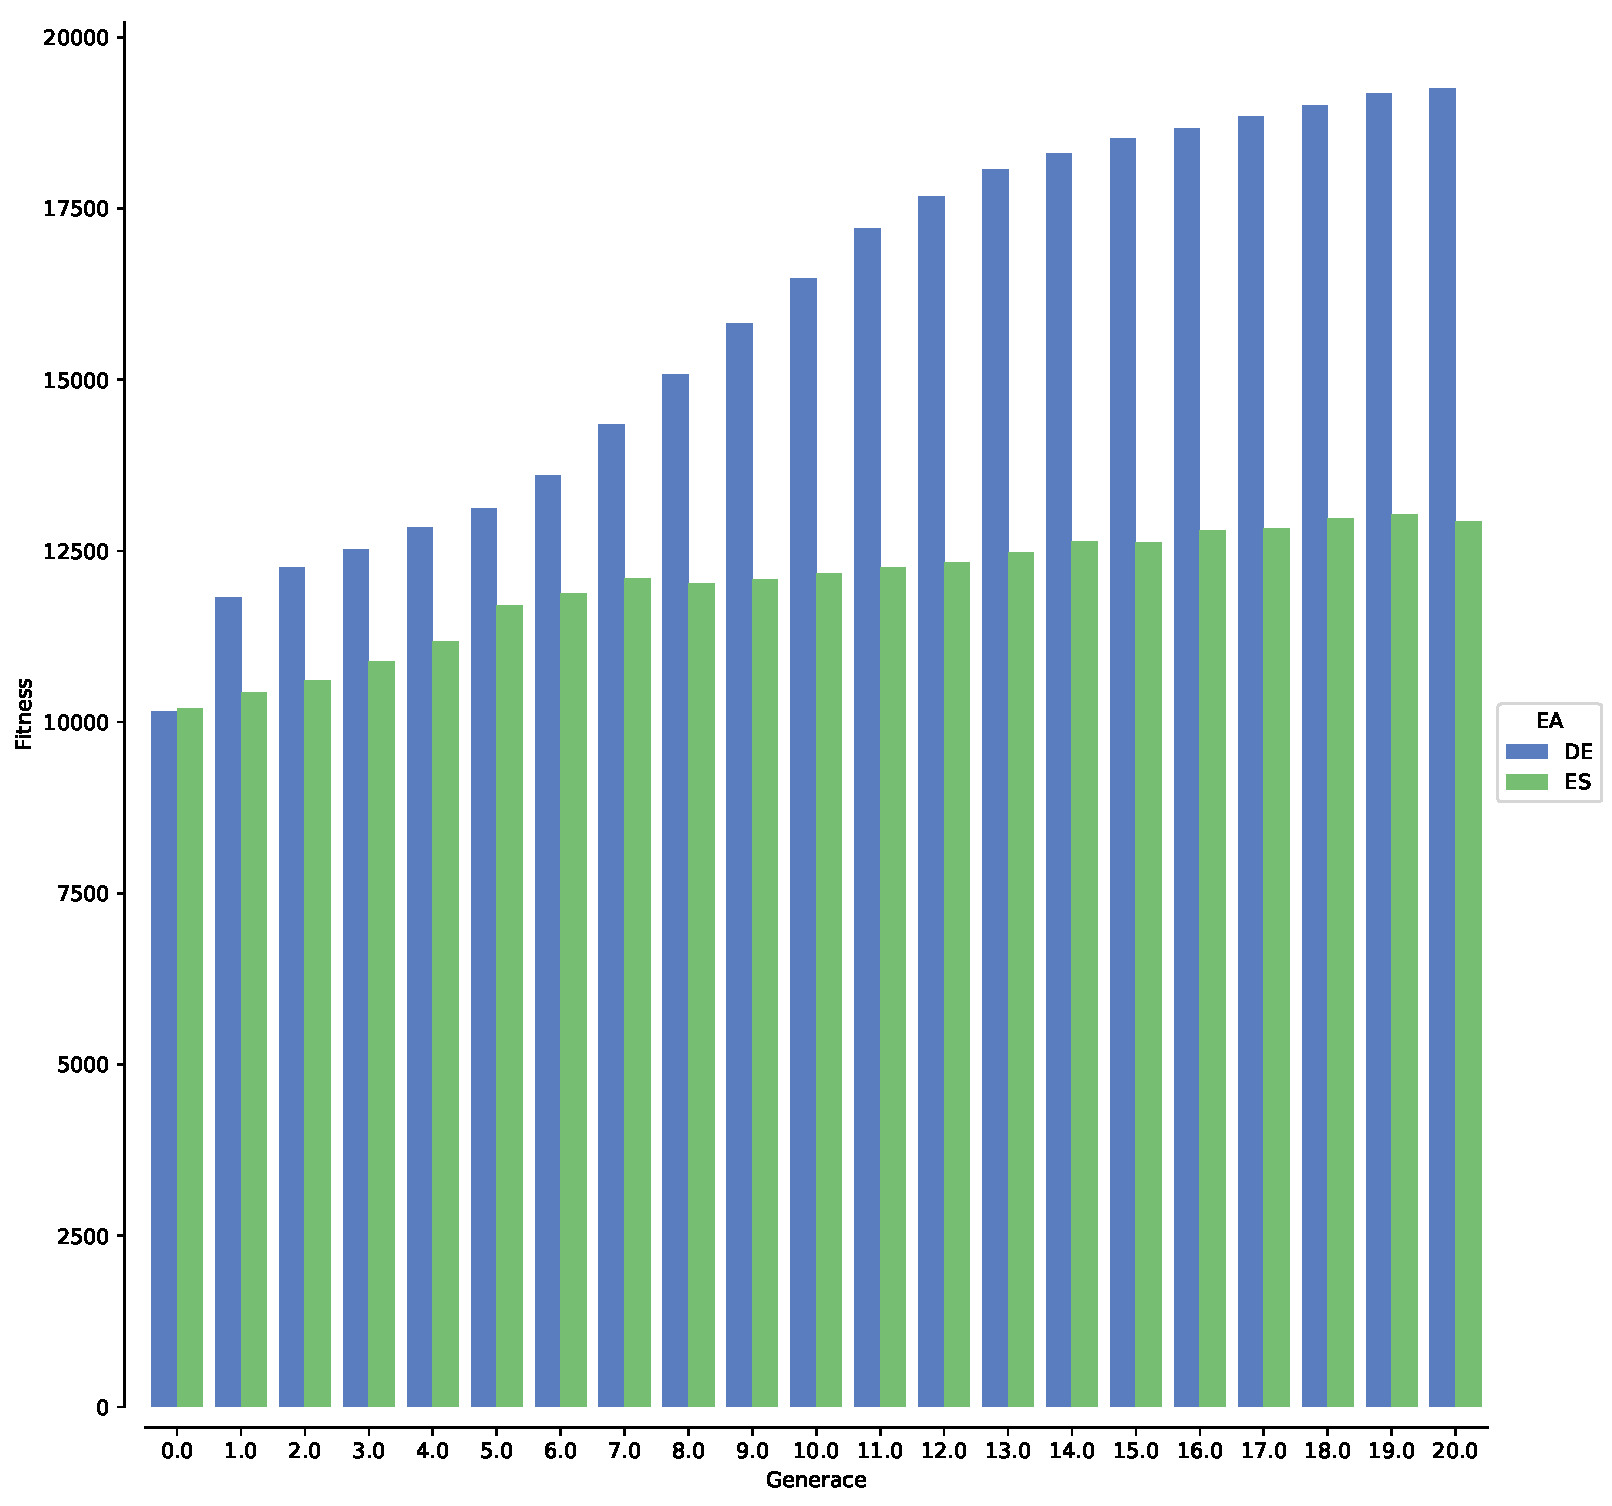
\includegraphics[width=\columnwidth]{../img/WoodMap/DEvsES/WorkerStockMem}
		\caption{Worker ukládání doprostřed  - porovnání průměrné fitness ES a DE}
		\label{obr04:StockESvsDE}
	\end{figure}
	\redo{Opravit obrázky
	}\begin{figure}[p]
		\centering
		\begin{subfigure}{.5\textwidth}
			\centering
			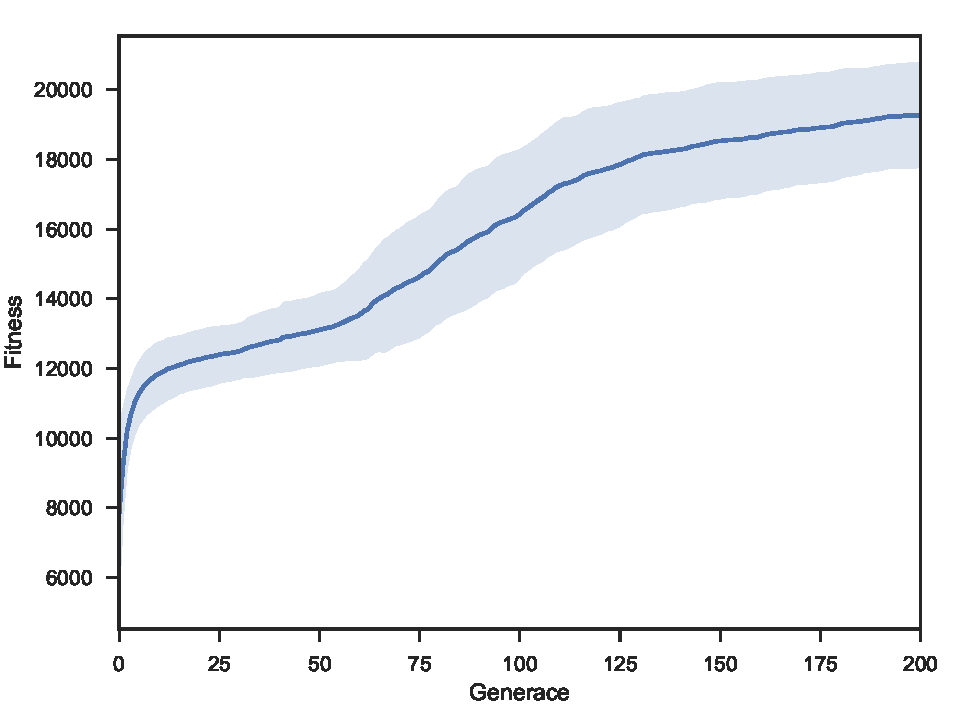
\includegraphics[width=\linewidth]{../img/WoodMap/DE/WorkerStockMem}
			\caption{DE}
			\label{obr04:StockDE}
		\end{subfigure}%
		\begin{subfigure}{.5\textwidth}
			\centering
			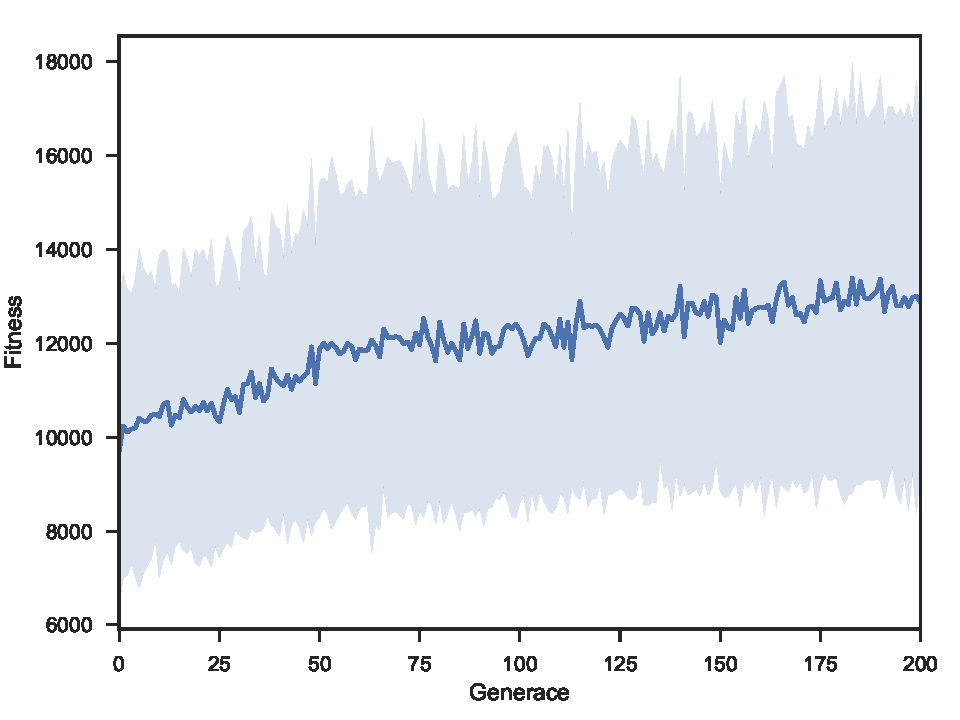
\includegraphics[width=\linewidth]{../img/WoodMap/ES/WoodStockES}
			\caption{ES}
			\label{obr04:StockES}
		\end{subfigure}
		\caption{Worker ukládání doprostřed  - Průběh fitness v rámci generací}
		\label{obr04:Stock}
	\end{figure}
	\clearpage
	\subsubsection{Kooperace  hlavní úkol  - nastavení experimentu}
	\begin{table}[h]\centering   
		\begin{tabular}{l@{\hspace{1.5cm}}D{.}{,}{3.2}D{.}{,}{1.2}D{.}{,}{2.3}}
			\toprule
			& \mc{} & \mc{}\\
			\pulrad{\textbf{Vlastnost:}} & \mc{\pulrad{\textbf{Hodnota:}}}\\
			\midrule
			Roboti: & Scout-5, Worker-4 \\
			Počet generací: & 4000\\
			Počet iterací map & 2000\\
			Velikost generace(DE) & 200\\
			Počet jedinců(ES) & 10\\
			Počet mutovaný potomků(ES)&20\\
			Elitismus(ES)& Ano\\
			Elitismus(DE)& Ne \\
			\bottomrule
			\multicolumn{2}{l}{}
		\end{tabular}
		\par 
		\begin{tabular}{l@{\hspace{1.5cm}}D{.}{,}{3.2}D{.}{,}{1.2}D{.}{,}{2.3}}
			\toprule
			& \mc{} & \mc{}\\
			\pulrad{\textbf{Vlastnost:}} & \mc{\pulrad{\textbf{Hodnota:}}}\\
			\midrule
			Hodnota nalezeného pokáceného stromu &  100 \\
			Hodnota uloženého dřeva & 1000\\
			Hodnota dřeva v kontejneru & 100\\
			Hodnota jiné entity v kontejneru & -100\\
			Hodnota kolize & -1\\
			Ostatní hodnoty: & 0\\
			Počet stromů: & 400\\
			Počet už pokácených stromů & 0\\
			\bottomrule
			\multicolumn{2}{l}{}
		\end{tabular}
			\caption{Kooperace  hlavní úkol  - nastavení experimentu}
	\end{table}
	\redo{Opravit obrázky}
	\clearpage
	
		\begin{figure}[t]\centering
		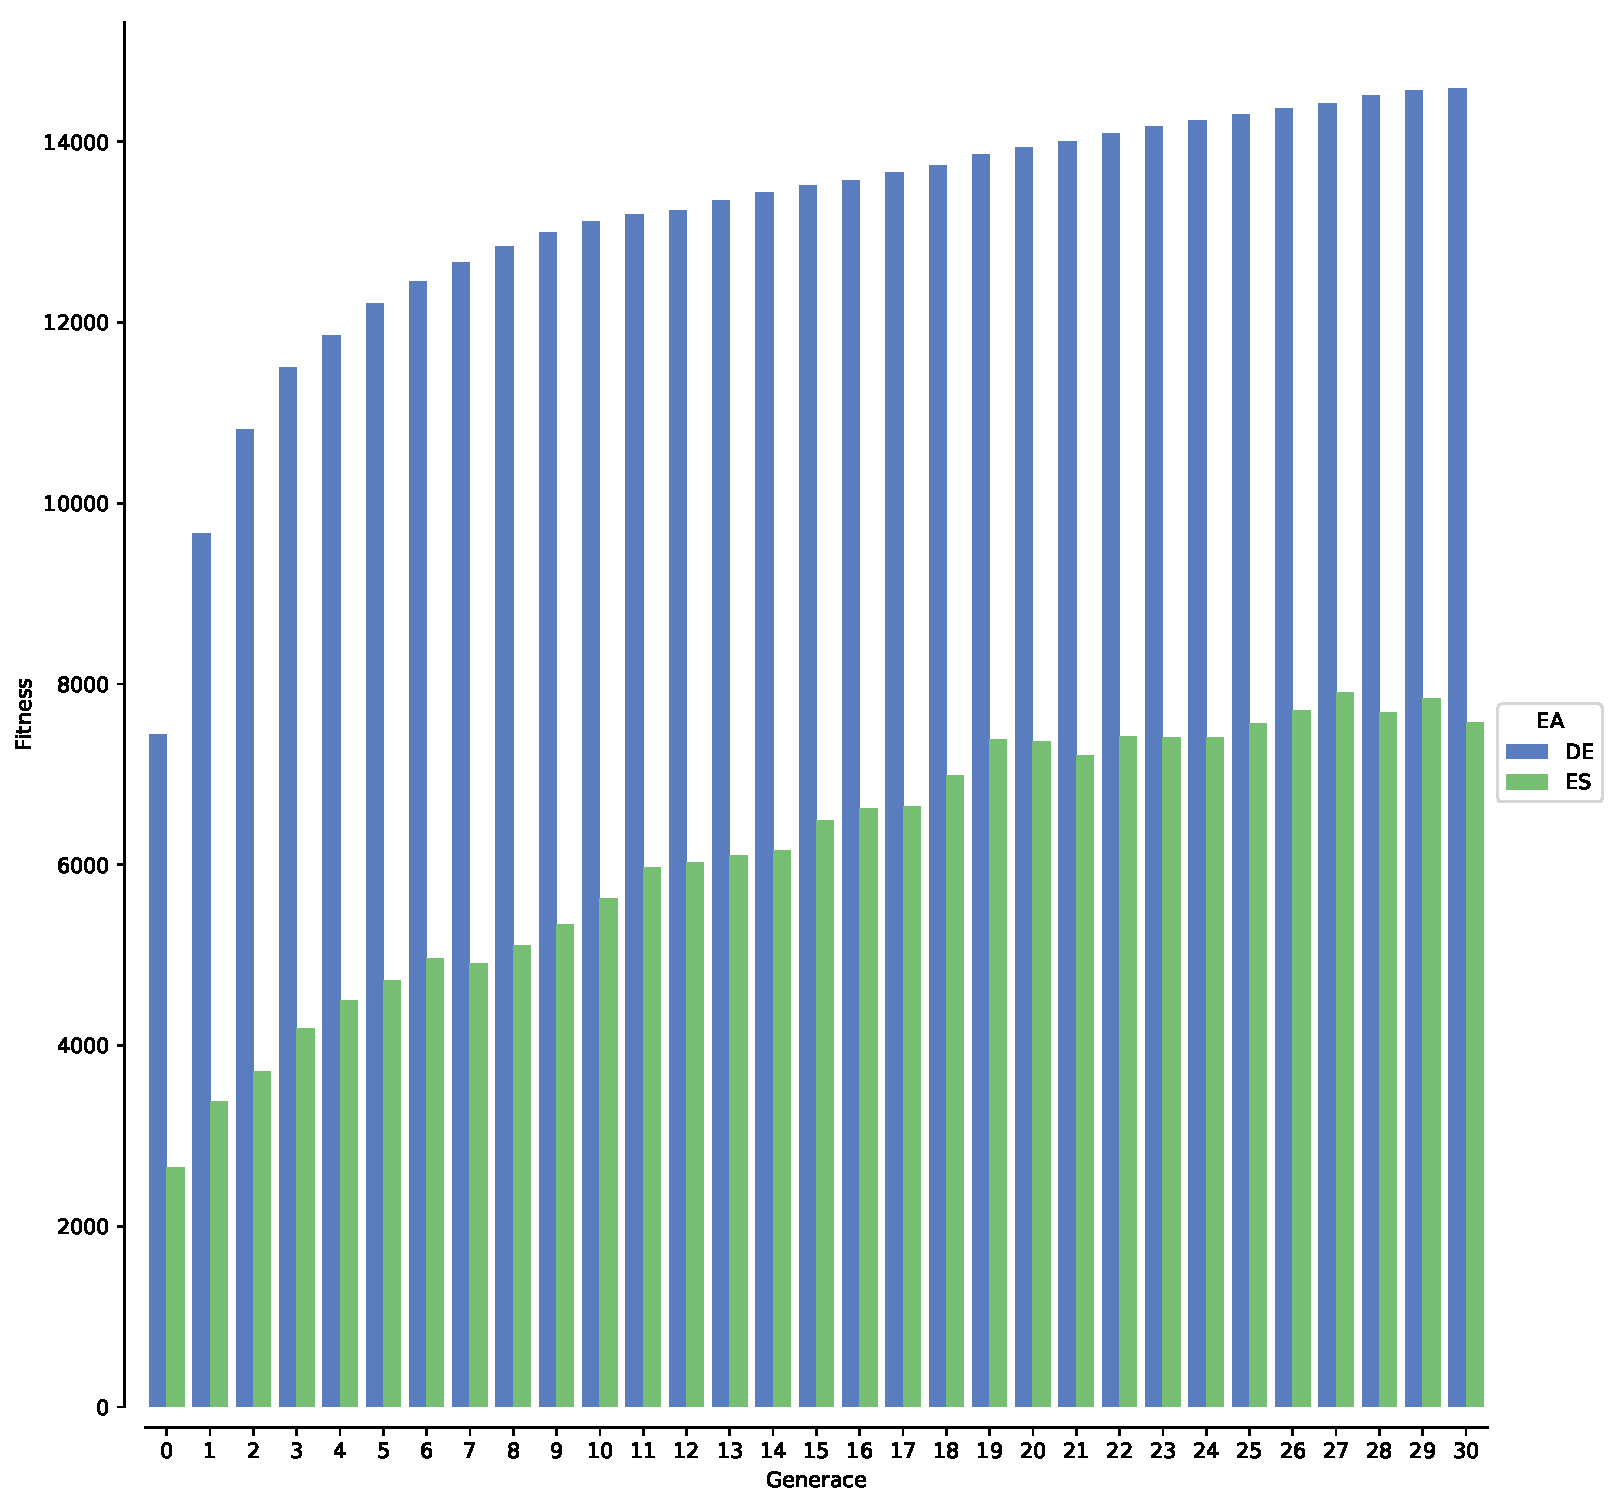
\includegraphics[width=\columnwidth]{../img/WoodMap/DEvsES/WoodCoopMem}
		\caption{Kooperace  hlavní úkol  - porovnání průměrné fitness ES a DE}
		\label{obr04:CoopESvsDE}
	\end{figure}
	\begin{figure}[p]
		\centering
		\begin{subfigure}{.5\textwidth}
			\centering
			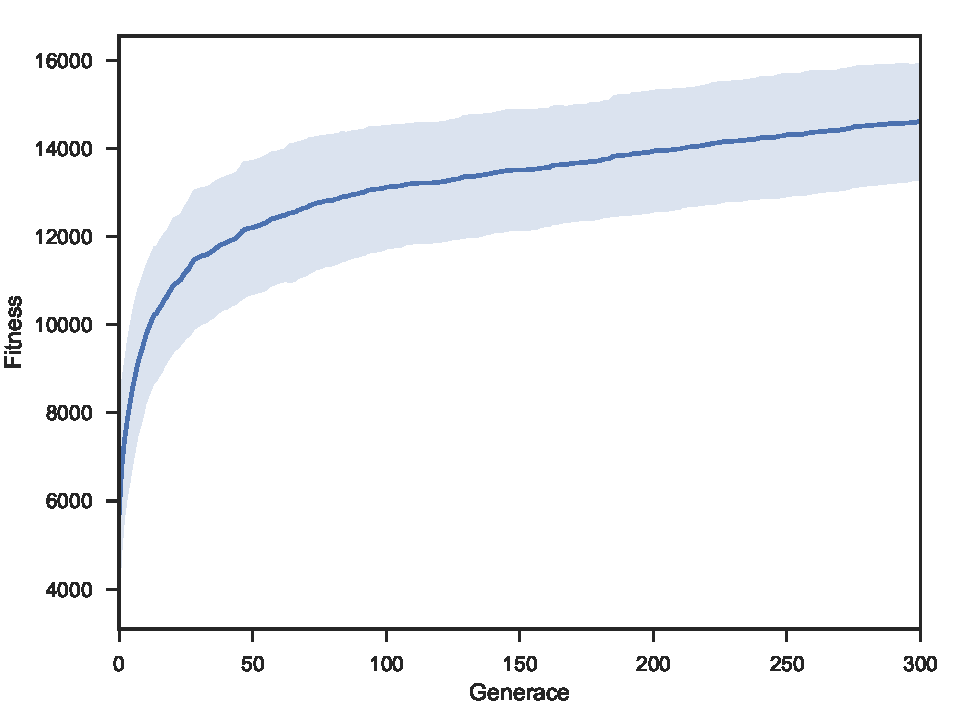
\includegraphics[width=\linewidth]{../img/WoodMap/DE/WoodCoopMem}
			\caption{DE}
			\label{obr04:CoopDE}
		\end{subfigure}%
		\begin{subfigure}{.5\textwidth}
			\centering
			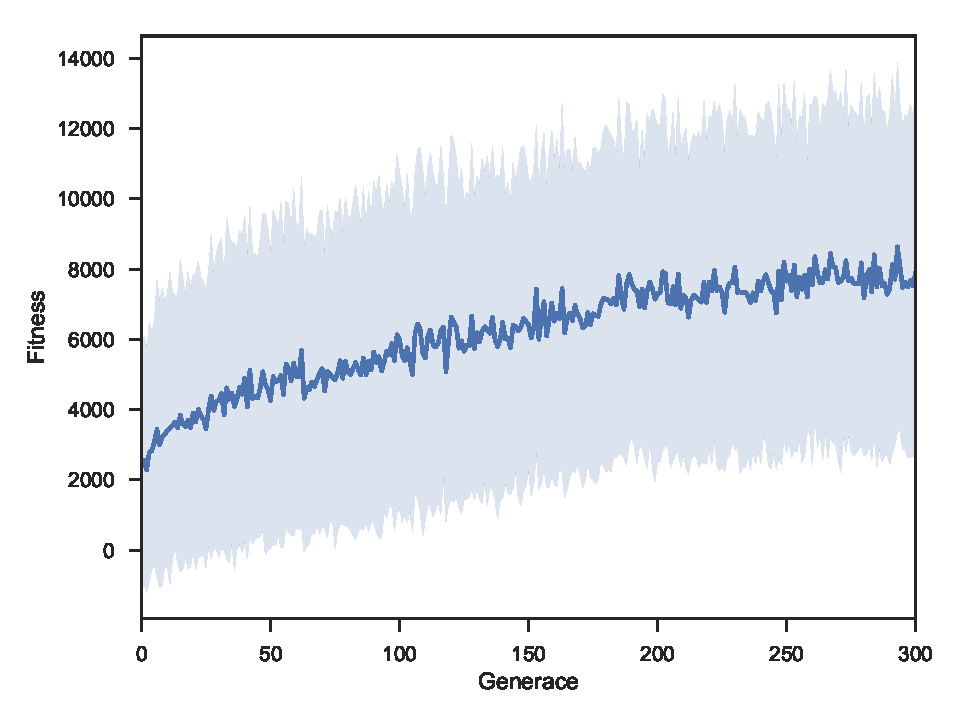
\includegraphics[width=\linewidth]{../img/WoodMap/ES/WoodCoopES}
			\caption{ES}
			\label{obr04:CoopES}
		\end{subfigure}
		\caption{Kooperace  hlavní úkol  - průběh fitness v rámci generací}
		\label{obr04:Coop}
	\end{figure}
	\clearpage
	
	\subsection{Výsledky Experimentu}
	Výsledkem posloupnosti všech podúkolů vzniklo poměrně velmi komplexní chování. Finální neuronové sítě ať u Worker robotů, či Scout robotů se zvládají vyhýbat překážkám. Scout roboti kácí stromy, které naleznou. Worker roboti nakládají zpracované dřevo, pokud na něj narazí, když zachytí signál úložiště, tak vyloží aktuální náklad. Některá chování byla také schopna předejít zaseknutí o nějaký shluk objektů, pokud byl  jejich pohyb vpřed neúspěšný, tak po několika pokusech roboti vycouvali a vydali se cestou okolo kritického místa. U většiny se také objevilo použití rádiových signálů jako prostředku pro největší možné rozptýlení po mapě, jakmile zachytí cizí signál vydají se opačným směrem. Průběh fitness jednotlivých podúkolů je zachycena na předchozích grafech \ref{obr04:Walk} až \ref{obr04:StockES}. 
	
	Ač se jedná o nejlepší dosažené chování objevují se nějaké nedostatky. Worker robot se občas dostane do pozice, ze které není schopen vyjet, jedná se především o kolize s vícero entitami. Tento problém by mohlo vyřešit použití vícevrstvých sítí či evolučního algoritmu evolvujícího i architekturu sítě. Skládání zpracovaného materiálu po obvodu skladiště není efektivní způsob, jak do něj naskládat maximální množství dřeva. V tomto případě jsem se snažil vylepšit tento nedostatek promítnutím vzdálenosti dřeva od středu skladiště do celkové fitness, ovšem bez znatelného zlepšení v chování. Nejspíše by bylo třeba použít rádiový senzor poskytující více informací o směru k zachycenému signálu. 
	\newpage 
	\begin{figure}[p]\centering
		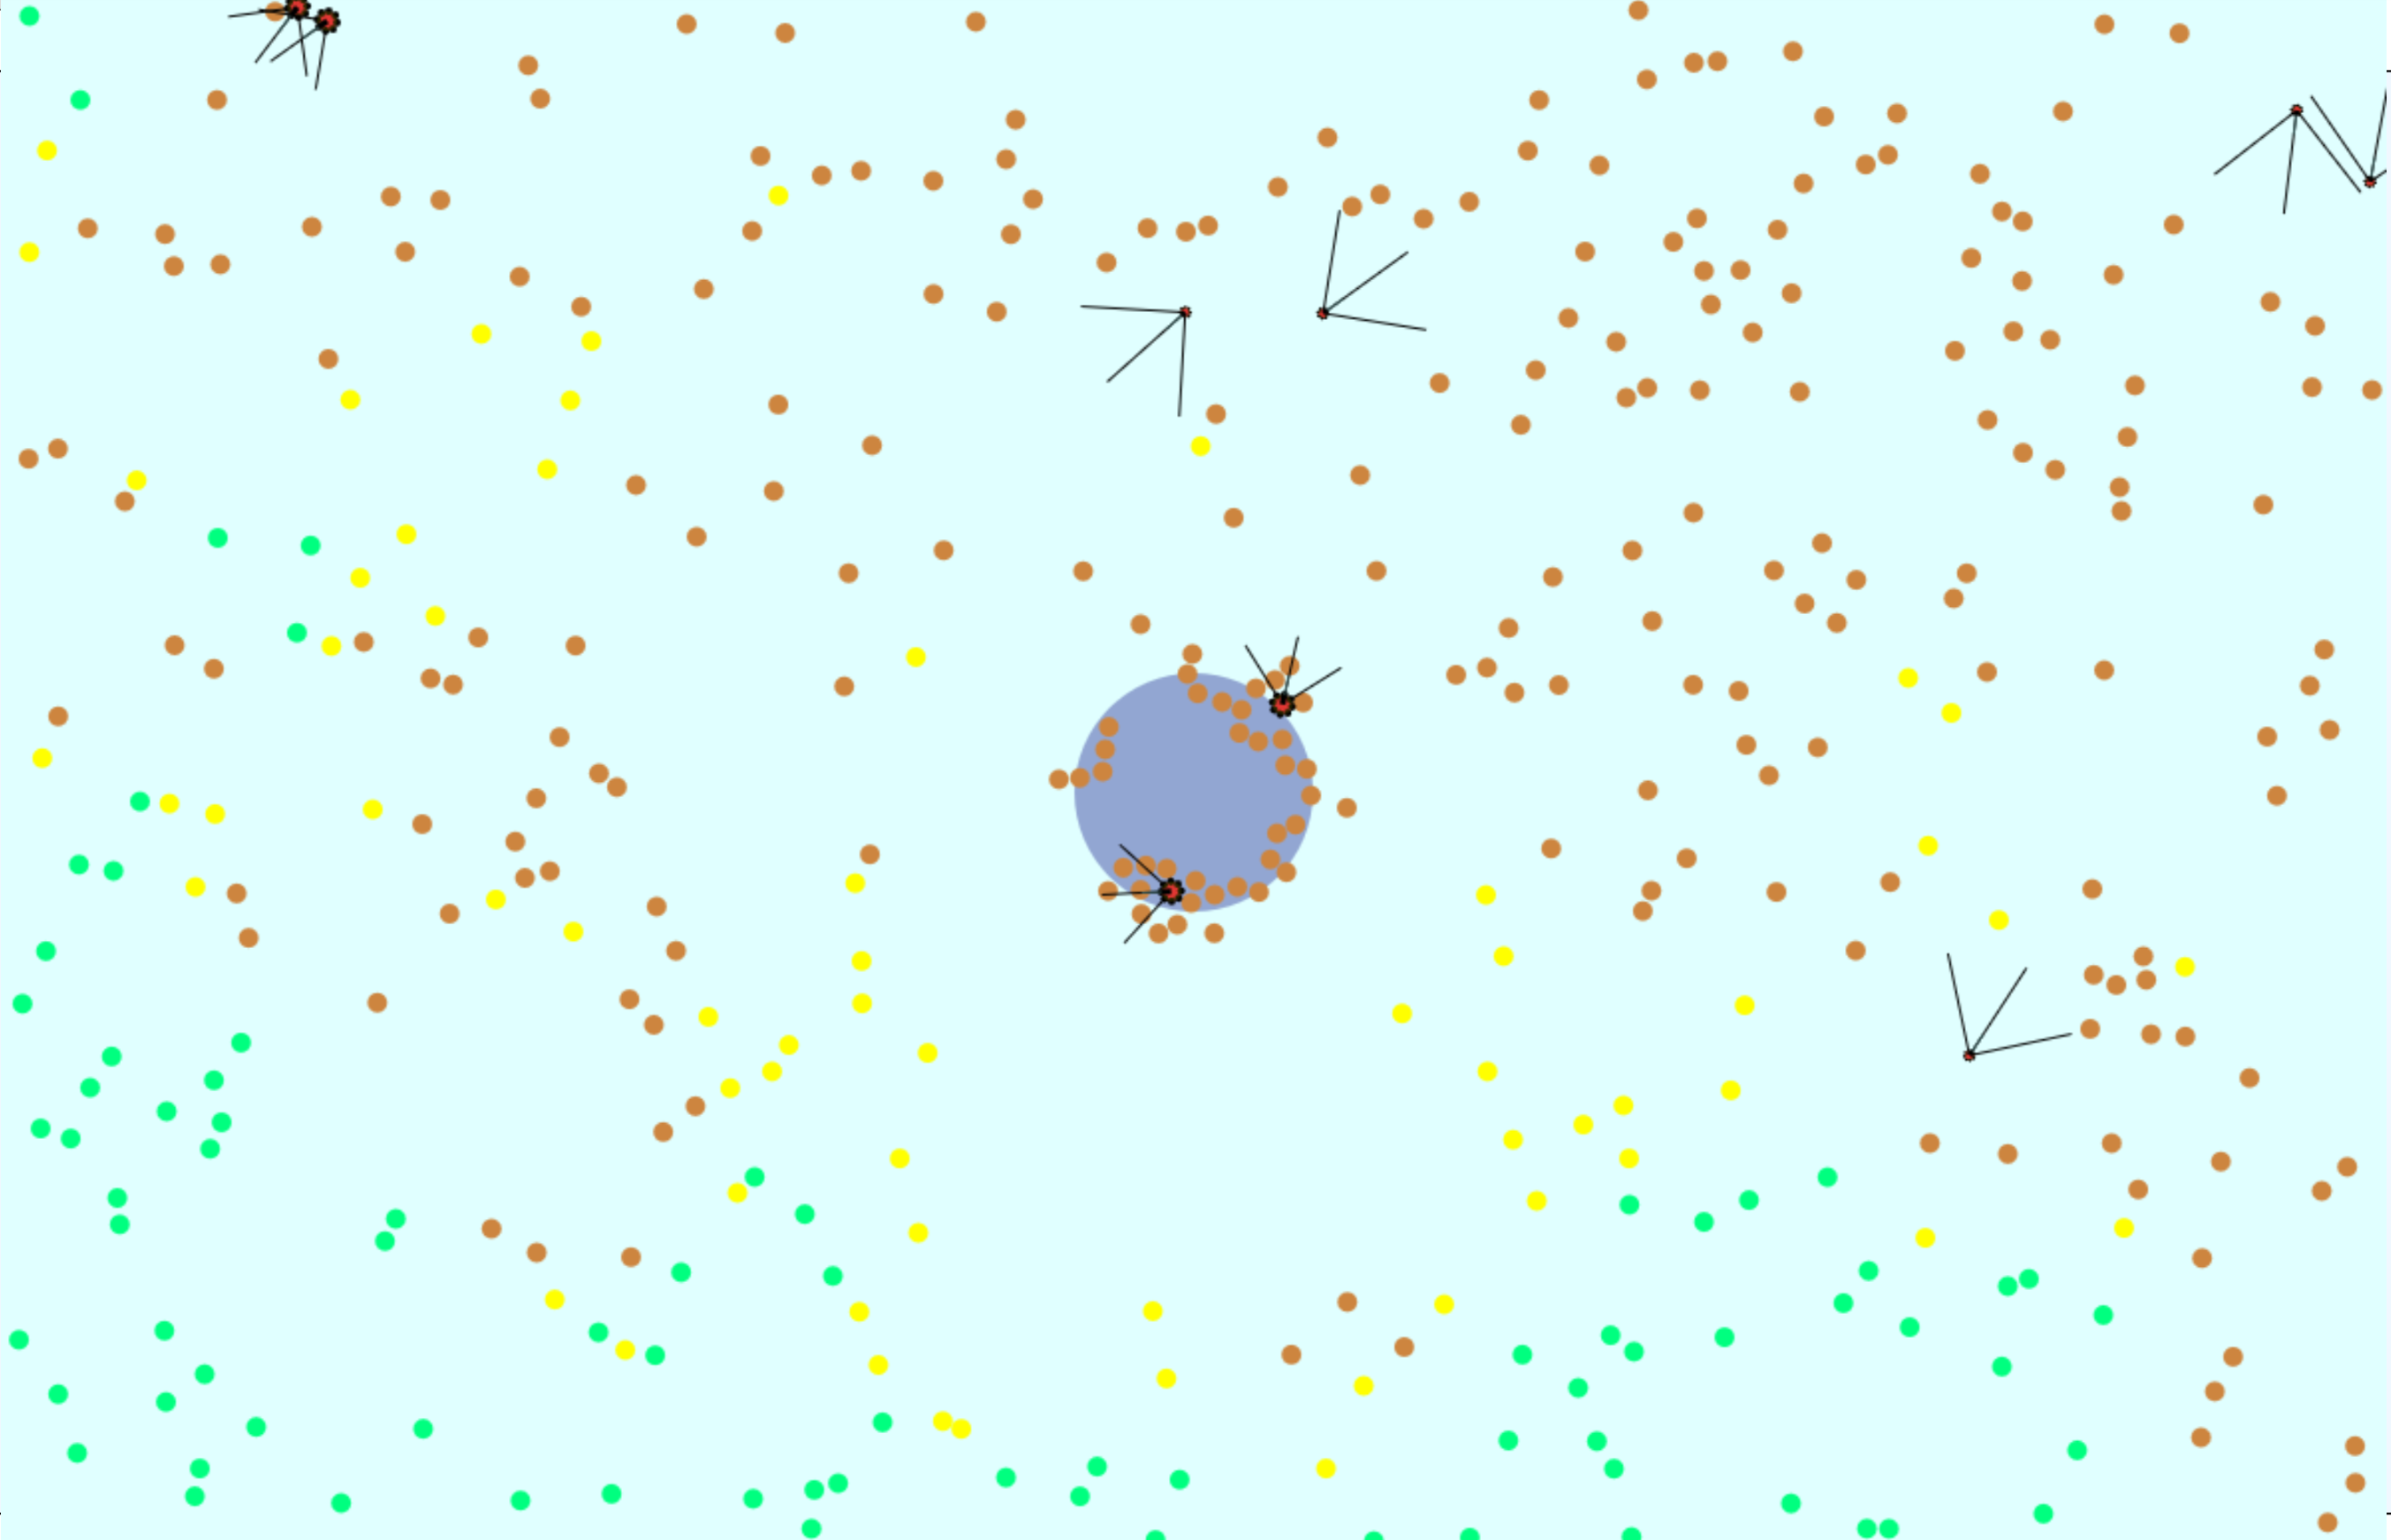
\includegraphics[width=\columnwidth]{../img/WoodMap/pictures/end.png}
		\caption{Nejlepší jedinec - 10000 iterací}
		\label{obr04:bestEnd}
	\end{figure}
	\begin{figure}[p]\centering
		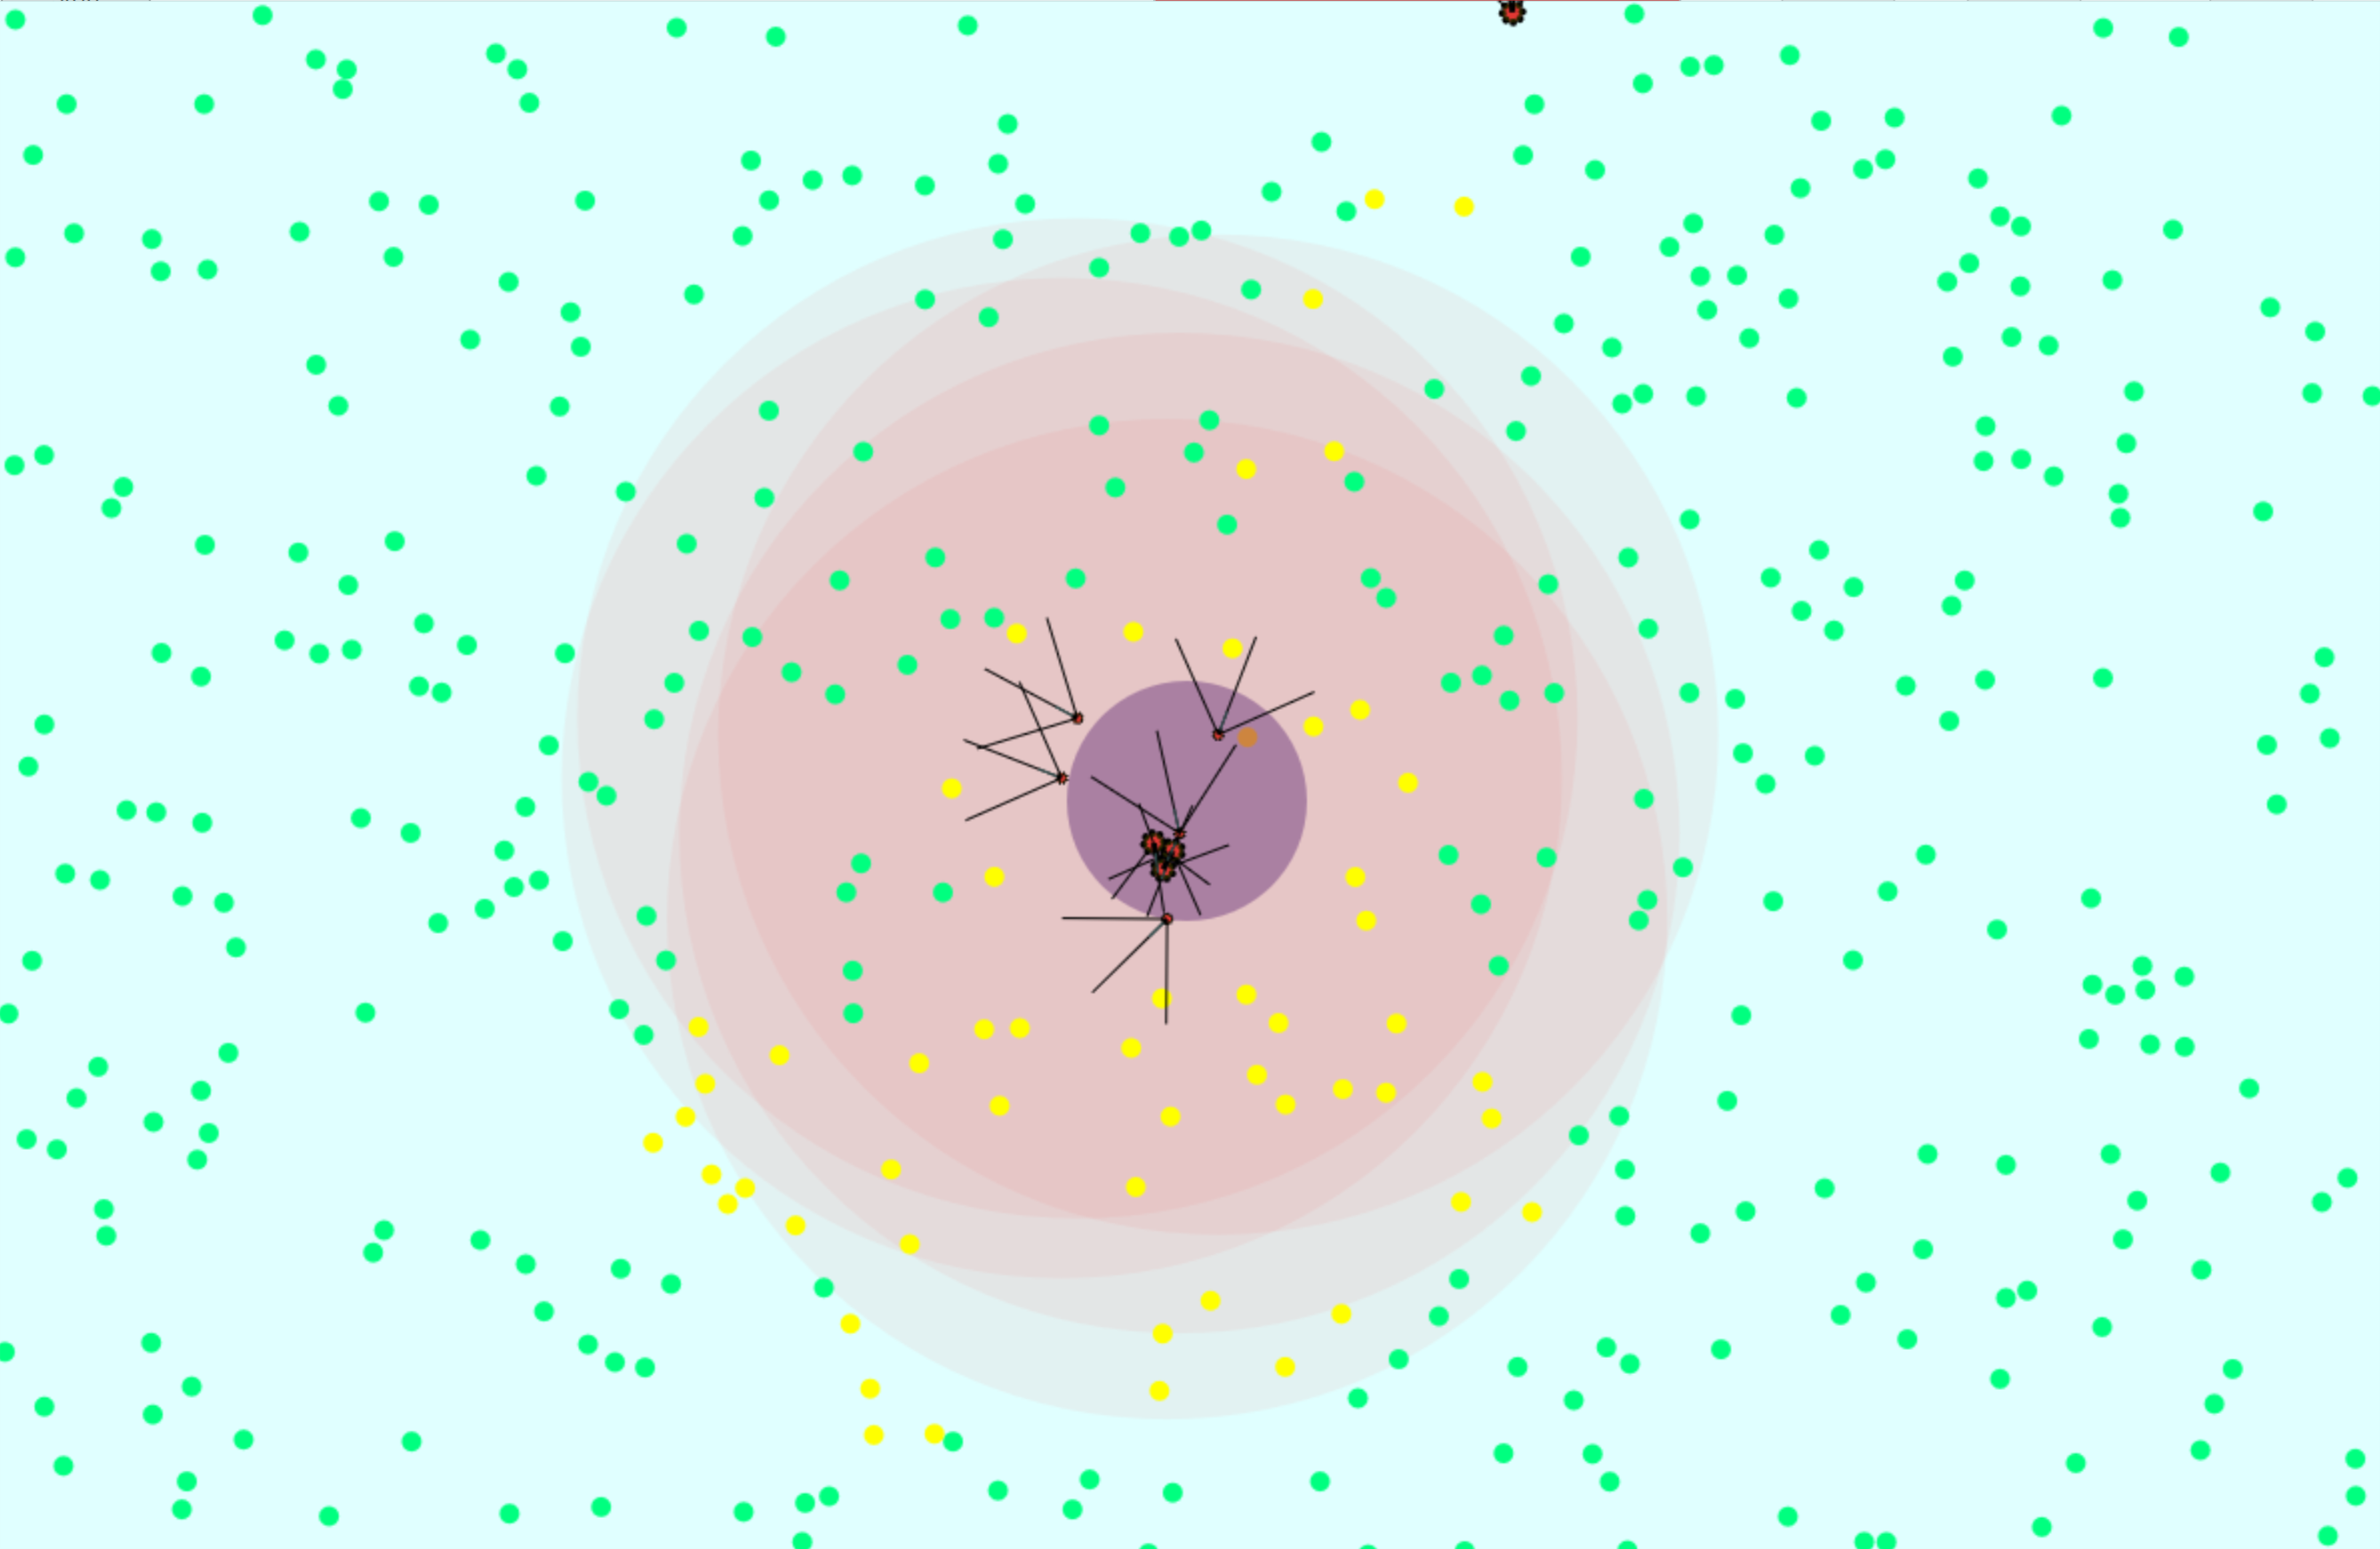
\includegraphics[width=\columnwidth]{../img/WoodMap/pictures/EndRandom.png}
		\caption{Nejlepší jedinec - 10000 iterací}
		\label{obr04:randomEnd}
	\end{figure}
	\clearpage
	\begin{table}[h]\centering   
		\begin{tabular}{l@{\hspace{1.5cm}}D{.}{,}{3.2}D{.}{,}{1.2}D{.}{,}{2.3}}
			\toprule
			& \mc{} & \mc{}\\
			Inicializační nastavení:  \\
			\midrule
			Výška & 800\\ 
			Šířka & 1200\\
			Počet iterací & 10000\\
			Počet stromů & 400\\
			Počet Scout robotů & 5\\
			Počet Worker robotů & 4\\
			\bottomrule
			\multicolumn{2}{l}{}
		\end{tabular}
		\caption{WoodScene - nastavení mapy pro statistické údaje}
	\end{table}
	\begin{table}[h]\centering   
		\begin{tabular}{l@{\hspace{1.5cm}}D{.}{,}{3.2}D{.}{,}{1.2}D{.}{,}{2.3}}
			\toprule
			& \mc{} & \mc{}\\
			Výsledky \\
			\bottomrule
			Zpracované dřevo zanechané v mapě & 225.22\\
			Stromy v mapě & 156.22\\
			Z toho nalezené & 52.84\\
			Dřevo v kontejnerech & 18.48\\
			Uskladněné dřevo & 17.56\\
			\multicolumn{2}{l}{}
		\end{tabular}
		\caption{WoodScene - průměrné výsledky nejlepšího chování pro 100 pokusů}
	\end{table}
	\paragraph{Shrnutí}
	\redo{Nějak shrnout, úplně nevím, co  by to mělo obsahovat.}
	\newpage

\redo{Předělat na stejný formát jako předchozí kapitola}
\section{Mineral Scene}
Jedná se o scénář reprezentující sběr surovin pro výrobu paliva a jeho následné využití. Figurují zde 3 rozliční roboti, všichni potřebují pro pohyb  dané množství paliva. Úspěšnost daného hejna se měří množstvím paliva. Nejmenší robot(Mineral scout) disponuje pouze senzory k exploraci prostředí a rádiovým vysílačem pro komunikaci se skupinou. Robot prostřední velikosti(Mineral Worker) se pohybuje o něco pomaleji než Mineral Scout, ale umí přesouvat objekty i více najednou. Robot pro přeměnu minerálu(,suroviny na výrobu paliva,) označen ve frameworku jako Mineral Refactor se přemisťuje nejpomaleji, má možnost přeměnit minerál na palivo. Tento scénář si bere jako inspiraci strategické hry a hypotetické přežití robotů na cizí planetě, kde si budou muset obstarat vlastní 
nerostné suroviny pro běh.

\section{Competitive Scene}
Poslední ze scénářů se týká soutěže dvou týmů(hejn) ve kterých figurují jeden malý průzkumný robot(Competitive Scout) a jeden vetší bojový robot(Competitive Fighter). Úspěšnost týmu je dána zachovanými jednotkami zdraví robotů a uděleným poškozením do nepřátelské skupiny robotů. Competitive Scout se pohybuje značně rychleji než Competitive Fighter, ale uděluje menší poškození. Což lze opět vztáhnout na chování rozdílných skupin nepřátel např. ve strategických hrách, kde se jejich chování adaptuje, co nejlépe na dané prostředí. 